
\documentclass[10pt]{article} % For LaTeX2e
\usepackage{tmlr}
% If accepted, instead use the following line for the camera-ready submission:
%\usepackage[accepted]{tmlr}
% To de-anonymize and remove mentions to TMLR (for example for posting to preprint servers), instead use the following:
%\usepackage[preprint]{tmlr}

% Optional math commands from https://github.com/goodfeli/dlbook_notation.
%%%%% NEW MATH DEFINITIONS %%%%%

\usepackage{amsmath,amsfonts,bm}

% Mark sections of captions for referring to divisions of figures
\newcommand{\figleft}{{\em (Left)}}
\newcommand{\figcenter}{{\em (Center)}}
\newcommand{\figright}{{\em (Right)}}
\newcommand{\figtop}{{\em (Top)}}
\newcommand{\figbottom}{{\em (Bottom)}}
\newcommand{\captiona}{{\em (a)}}
\newcommand{\captionb}{{\em (b)}}
\newcommand{\captionc}{{\em (c)}}
\newcommand{\captiond}{{\em (d)}}

% Highlight a newly defined term
\newcommand{\newterm}[1]{{\bf #1}}


% Figure reference, lower-case.
\def\figref#1{figure~\ref{#1}}
% Figure reference, capital. For start of sentence
\def\Figref#1{Figure~\ref{#1}}
\def\twofigref#1#2{figures \ref{#1} and \ref{#2}}
\def\quadfigref#1#2#3#4{figures \ref{#1}, \ref{#2}, \ref{#3} and \ref{#4}}
% Section reference, lower-case.
\def\secref#1{section~\ref{#1}}
% Section reference, capital.
\def\Secref#1{Section~\ref{#1}}
% Reference to two sections.
\def\twosecrefs#1#2{sections \ref{#1} and \ref{#2}}
% Reference to three sections.
\def\secrefs#1#2#3{sections \ref{#1}, \ref{#2} and \ref{#3}}
% Reference to an equation, lower-case.
\def\eqref#1{equation~\ref{#1}}
% Reference to an equation, upper case
\def\Eqref#1{Equation~\ref{#1}}
% A raw reference to an equation---avoid using if possible
\def\plaineqref#1{\ref{#1}}
% Reference to a chapter, lower-case.
\def\chapref#1{chapter~\ref{#1}}
% Reference to an equation, upper case.
\def\Chapref#1{Chapter~\ref{#1}}
% Reference to a range of chapters
\def\rangechapref#1#2{chapters\ref{#1}--\ref{#2}}
% Reference to an algorithm, lower-case.
\def\algref#1{algorithm~\ref{#1}}
% Reference to an algorithm, upper case.
\def\Algref#1{Algorithm~\ref{#1}}
\def\twoalgref#1#2{algorithms \ref{#1} and \ref{#2}}
\def\Twoalgref#1#2{Algorithms \ref{#1} and \ref{#2}}
% Reference to a part, lower case
\def\partref#1{part~\ref{#1}}
% Reference to a part, upper case
\def\Partref#1{Part~\ref{#1}}
\def\twopartref#1#2{parts \ref{#1} and \ref{#2}}

\def\ceil#1{\lceil #1 \rceil}
\def\floor#1{\lfloor #1 \rfloor}
\def\1{\bm{1}}
\newcommand{\train}{\mathcal{D}}
\newcommand{\valid}{\mathcal{D_{\mathrm{valid}}}}
\newcommand{\test}{\mathcal{D_{\mathrm{test}}}}

\def\eps{{\epsilon}}


% Random variables
\def\reta{{\textnormal{$\eta$}}}
\def\ra{{\textnormal{a}}}
\def\rb{{\textnormal{b}}}
\def\rc{{\textnormal{c}}}
\def\rd{{\textnormal{d}}}
\def\re{{\textnormal{e}}}
\def\rf{{\textnormal{f}}}
\def\rg{{\textnormal{g}}}
\def\rh{{\textnormal{h}}}
\def\ri{{\textnormal{i}}}
\def\rj{{\textnormal{j}}}
\def\rk{{\textnormal{k}}}
\def\rl{{\textnormal{l}}}
% rm is already a command, just don't name any random variables m
\def\rn{{\textnormal{n}}}
\def\ro{{\textnormal{o}}}
\def\rp{{\textnormal{p}}}
\def\rq{{\textnormal{q}}}
\def\rr{{\textnormal{r}}}
\def\rs{{\textnormal{s}}}
\def\rt{{\textnormal{t}}}
\def\ru{{\textnormal{u}}}
\def\rv{{\textnormal{v}}}
\def\rw{{\textnormal{w}}}
\def\rx{{\textnormal{x}}}
\def\ry{{\textnormal{y}}}
\def\rz{{\textnormal{z}}}

% Random vectors
\def\rvepsilon{{\mathbf{\epsilon}}}
\def\rvtheta{{\mathbf{\theta}}}
\def\rva{{\mathbf{a}}}
\def\rvb{{\mathbf{b}}}
\def\rvc{{\mathbf{c}}}
\def\rvd{{\mathbf{d}}}
\def\rve{{\mathbf{e}}}
\def\rvf{{\mathbf{f}}}
\def\rvg{{\mathbf{g}}}
\def\rvh{{\mathbf{h}}}
\def\rvu{{\mathbf{i}}}
\def\rvj{{\mathbf{j}}}
\def\rvk{{\mathbf{k}}}
\def\rvl{{\mathbf{l}}}
\def\rvm{{\mathbf{m}}}
\def\rvn{{\mathbf{n}}}
\def\rvo{{\mathbf{o}}}
\def\rvp{{\mathbf{p}}}
\def\rvq{{\mathbf{q}}}
\def\rvr{{\mathbf{r}}}
\def\rvs{{\mathbf{s}}}
\def\rvt{{\mathbf{t}}}
\def\rvu{{\mathbf{u}}}
\def\rvv{{\mathbf{v}}}
\def\rvw{{\mathbf{w}}}
\def\rvx{{\mathbf{x}}}
\def\rvy{{\mathbf{y}}}
\def\rvz{{\mathbf{z}}}

% Elements of random vectors
\def\erva{{\textnormal{a}}}
\def\ervb{{\textnormal{b}}}
\def\ervc{{\textnormal{c}}}
\def\ervd{{\textnormal{d}}}
\def\erve{{\textnormal{e}}}
\def\ervf{{\textnormal{f}}}
\def\ervg{{\textnormal{g}}}
\def\ervh{{\textnormal{h}}}
\def\ervi{{\textnormal{i}}}
\def\ervj{{\textnormal{j}}}
\def\ervk{{\textnormal{k}}}
\def\ervl{{\textnormal{l}}}
\def\ervm{{\textnormal{m}}}
\def\ervn{{\textnormal{n}}}
\def\ervo{{\textnormal{o}}}
\def\ervp{{\textnormal{p}}}
\def\ervq{{\textnormal{q}}}
\def\ervr{{\textnormal{r}}}
\def\ervs{{\textnormal{s}}}
\def\ervt{{\textnormal{t}}}
\def\ervu{{\textnormal{u}}}
\def\ervv{{\textnormal{v}}}
\def\ervw{{\textnormal{w}}}
\def\ervx{{\textnormal{x}}}
\def\ervy{{\textnormal{y}}}
\def\ervz{{\textnormal{z}}}

% Random matrices
\def\rmA{{\mathbf{A}}}
\def\rmB{{\mathbf{B}}}
\def\rmC{{\mathbf{C}}}
\def\rmD{{\mathbf{D}}}
\def\rmE{{\mathbf{E}}}
\def\rmF{{\mathbf{F}}}
\def\rmG{{\mathbf{G}}}
\def\rmH{{\mathbf{H}}}
\def\rmI{{\mathbf{I}}}
\def\rmJ{{\mathbf{J}}}
\def\rmK{{\mathbf{K}}}
\def\rmL{{\mathbf{L}}}
\def\rmM{{\mathbf{M}}}
\def\rmN{{\mathbf{N}}}
\def\rmO{{\mathbf{O}}}
\def\rmP{{\mathbf{P}}}
\def\rmQ{{\mathbf{Q}}}
\def\rmR{{\mathbf{R}}}
\def\rmS{{\mathbf{S}}}
\def\rmT{{\mathbf{T}}}
\def\rmU{{\mathbf{U}}}
\def\rmV{{\mathbf{V}}}
\def\rmW{{\mathbf{W}}}
\def\rmX{{\mathbf{X}}}
\def\rmY{{\mathbf{Y}}}
\def\rmZ{{\mathbf{Z}}}

% Elements of random matrices
\def\ermA{{\textnormal{A}}}
\def\ermB{{\textnormal{B}}}
\def\ermC{{\textnormal{C}}}
\def\ermD{{\textnormal{D}}}
\def\ermE{{\textnormal{E}}}
\def\ermF{{\textnormal{F}}}
\def\ermG{{\textnormal{G}}}
\def\ermH{{\textnormal{H}}}
\def\ermI{{\textnormal{I}}}
\def\ermJ{{\textnormal{J}}}
\def\ermK{{\textnormal{K}}}
\def\ermL{{\textnormal{L}}}
\def\ermM{{\textnormal{M}}}
\def\ermN{{\textnormal{N}}}
\def\ermO{{\textnormal{O}}}
\def\ermP{{\textnormal{P}}}
\def\ermQ{{\textnormal{Q}}}
\def\ermR{{\textnormal{R}}}
\def\ermS{{\textnormal{S}}}
\def\ermT{{\textnormal{T}}}
\def\ermU{{\textnormal{U}}}
\def\ermV{{\textnormal{V}}}
\def\ermW{{\textnormal{W}}}
\def\ermX{{\textnormal{X}}}
\def\ermY{{\textnormal{Y}}}
\def\ermZ{{\textnormal{Z}}}

% Vectors
\def\vzero{{\bm{0}}}
\def\vone{{\bm{1}}}
\def\vmu{{\bm{\mu}}}
\def\vtheta{{\bm{\theta}}}
\def\va{{\bm{a}}}
\def\vb{{\bm{b}}}
\def\vc{{\bm{c}}}
\def\vd{{\bm{d}}}
\def\ve{{\bm{e}}}
\def\vf{{\bm{f}}}
\def\vg{{\bm{g}}}
\def\vh{{\bm{h}}}
\def\vi{{\bm{i}}}
\def\vj{{\bm{j}}}
\def\vk{{\bm{k}}}
\def\vl{{\bm{l}}}
\def\vm{{\bm{m}}}
\def\vn{{\bm{n}}}
\def\vo{{\bm{o}}}
\def\vp{{\bm{p}}}
\def\vq{{\bm{q}}}
\def\vr{{\bm{r}}}
\def\vs{{\bm{s}}}
\def\vt{{\bm{t}}}
\def\vu{{\bm{u}}}
\def\vv{{\bm{v}}}
\def\vw{{\bm{w}}}
\def\vx{{\bm{x}}}
\def\vy{{\bm{y}}}
\def\vz{{\bm{z}}}

% Elements of vectors
\def\evalpha{{\alpha}}
\def\evbeta{{\beta}}
\def\evepsilon{{\epsilon}}
\def\evlambda{{\lambda}}
\def\evomega{{\omega}}
\def\evmu{{\mu}}
\def\evpsi{{\psi}}
\def\evsigma{{\sigma}}
\def\evtheta{{\theta}}
\def\eva{{a}}
\def\evb{{b}}
\def\evc{{c}}
\def\evd{{d}}
\def\eve{{e}}
\def\evf{{f}}
\def\evg{{g}}
\def\evh{{h}}
\def\evi{{i}}
\def\evj{{j}}
\def\evk{{k}}
\def\evl{{l}}
\def\evm{{m}}
\def\evn{{n}}
\def\evo{{o}}
\def\evp{{p}}
\def\evq{{q}}
\def\evr{{r}}
\def\evs{{s}}
\def\evt{{t}}
\def\evu{{u}}
\def\evv{{v}}
\def\evw{{w}}
\def\evx{{x}}
\def\evy{{y}}
\def\evz{{z}}

% Matrix
\def\mA{{\bm{A}}}
\def\mB{{\bm{B}}}
\def\mC{{\bm{C}}}
\def\mD{{\bm{D}}}
\def\mE{{\bm{E}}}
\def\mF{{\bm{F}}}
\def\mG{{\bm{G}}}
\def\mH{{\bm{H}}}
\def\mI{{\bm{I}}}
\def\mJ{{\bm{J}}}
\def\mK{{\bm{K}}}
\def\mL{{\bm{L}}}
\def\mM{{\bm{M}}}
\def\mN{{\bm{N}}}
\def\mO{{\bm{O}}}
\def\mP{{\bm{P}}}
\def\mQ{{\bm{Q}}}
\def\mR{{\bm{R}}}
\def\mS{{\bm{S}}}
\def\mT{{\bm{T}}}
\def\mU{{\bm{U}}}
\def\mV{{\bm{V}}}
\def\mW{{\bm{W}}}
\def\mX{{\bm{X}}}
\def\mY{{\bm{Y}}}
\def\mZ{{\bm{Z}}}
\def\mBeta{{\bm{\beta}}}
\def\mPhi{{\bm{\Phi}}}
\def\mLambda{{\bm{\Lambda}}}
\def\mSigma{{\bm{\Sigma}}}

% Tensor
\DeclareMathAlphabet{\mathsfit}{\encodingdefault}{\sfdefault}{m}{sl}
\SetMathAlphabet{\mathsfit}{bold}{\encodingdefault}{\sfdefault}{bx}{n}
\newcommand{\tens}[1]{\bm{\mathsfit{#1}}}
\def\tA{{\tens{A}}}
\def\tB{{\tens{B}}}
\def\tC{{\tens{C}}}
\def\tD{{\tens{D}}}
\def\tE{{\tens{E}}}
\def\tF{{\tens{F}}}
\def\tG{{\tens{G}}}
\def\tH{{\tens{H}}}
\def\tI{{\tens{I}}}
\def\tJ{{\tens{J}}}
\def\tK{{\tens{K}}}
\def\tL{{\tens{L}}}
\def\tM{{\tens{M}}}
\def\tN{{\tens{N}}}
\def\tO{{\tens{O}}}
\def\tP{{\tens{P}}}
\def\tQ{{\tens{Q}}}
\def\tR{{\tens{R}}}
\def\tS{{\tens{S}}}
\def\tT{{\tens{T}}}
\def\tU{{\tens{U}}}
\def\tV{{\tens{V}}}
\def\tW{{\tens{W}}}
\def\tX{{\tens{X}}}
\def\tY{{\tens{Y}}}
\def\tZ{{\tens{Z}}}


% Graph
\def\gA{{\mathcal{A}}}
\def\gB{{\mathcal{B}}}
\def\gC{{\mathcal{C}}}
\def\gD{{\mathcal{D}}}
\def\gE{{\mathcal{E}}}
\def\gF{{\mathcal{F}}}
\def\gG{{\mathcal{G}}}
\def\gH{{\mathcal{H}}}
\def\gI{{\mathcal{I}}}
\def\gJ{{\mathcal{J}}}
\def\gK{{\mathcal{K}}}
\def\gL{{\mathcal{L}}}
\def\gM{{\mathcal{M}}}
\def\gN{{\mathcal{N}}}
\def\gO{{\mathcal{O}}}
\def\gP{{\mathcal{P}}}
\def\gQ{{\mathcal{Q}}}
\def\gR{{\mathcal{R}}}
\def\gS{{\mathcal{S}}}
\def\gT{{\mathcal{T}}}
\def\gU{{\mathcal{U}}}
\def\gV{{\mathcal{V}}}
\def\gW{{\mathcal{W}}}
\def\gX{{\mathcal{X}}}
\def\gY{{\mathcal{Y}}}
\def\gZ{{\mathcal{Z}}}

% Sets
\def\sA{{\mathbb{A}}}
\def\sB{{\mathbb{B}}}
\def\sC{{\mathbb{C}}}
\def\sD{{\mathbb{D}}}
% Don't use a set called E, because this would be the same as our symbol
% for expectation.
\def\sF{{\mathbb{F}}}
\def\sG{{\mathbb{G}}}
\def\sH{{\mathbb{H}}}
\def\sI{{\mathbb{I}}}
\def\sJ{{\mathbb{J}}}
\def\sK{{\mathbb{K}}}
\def\sL{{\mathbb{L}}}
\def\sM{{\mathbb{M}}}
\def\sN{{\mathbb{N}}}
\def\sO{{\mathbb{O}}}
\def\sP{{\mathbb{P}}}
\def\sQ{{\mathbb{Q}}}
\def\sR{{\mathbb{R}}}
\def\sS{{\mathbb{S}}}
\def\sT{{\mathbb{T}}}
\def\sU{{\mathbb{U}}}
\def\sV{{\mathbb{V}}}
\def\sW{{\mathbb{W}}}
\def\sX{{\mathbb{X}}}
\def\sY{{\mathbb{Y}}}
\def\sZ{{\mathbb{Z}}}

% Entries of a matrix
\def\emLambda{{\Lambda}}
\def\emA{{A}}
\def\emB{{B}}
\def\emC{{C}}
\def\emD{{D}}
\def\emE{{E}}
\def\emF{{F}}
\def\emG{{G}}
\def\emH{{H}}
\def\emI{{I}}
\def\emJ{{J}}
\def\emK{{K}}
\def\emL{{L}}
\def\emM{{M}}
\def\emN{{N}}
\def\emO{{O}}
\def\emP{{P}}
\def\emQ{{Q}}
\def\emR{{R}}
\def\emS{{S}}
\def\emT{{T}}
\def\emU{{U}}
\def\emV{{V}}
\def\emW{{W}}
\def\emX{{X}}
\def\emY{{Y}}
\def\emZ{{Z}}
\def\emSigma{{\Sigma}}

% entries of a tensor
% Same font as tensor, without \bm wrapper
\newcommand{\etens}[1]{\mathsfit{#1}}
\def\etLambda{{\etens{\Lambda}}}
\def\etA{{\etens{A}}}
\def\etB{{\etens{B}}}
\def\etC{{\etens{C}}}
\def\etD{{\etens{D}}}
\def\etE{{\etens{E}}}
\def\etF{{\etens{F}}}
\def\etG{{\etens{G}}}
\def\etH{{\etens{H}}}
\def\etI{{\etens{I}}}
\def\etJ{{\etens{J}}}
\def\etK{{\etens{K}}}
\def\etL{{\etens{L}}}
\def\etM{{\etens{M}}}
\def\etN{{\etens{N}}}
\def\etO{{\etens{O}}}
\def\etP{{\etens{P}}}
\def\etQ{{\etens{Q}}}
\def\etR{{\etens{R}}}
\def\etS{{\etens{S}}}
\def\etT{{\etens{T}}}
\def\etU{{\etens{U}}}
\def\etV{{\etens{V}}}
\def\etW{{\etens{W}}}
\def\etX{{\etens{X}}}
\def\etY{{\etens{Y}}}
\def\etZ{{\etens{Z}}}

% The true underlying data generating distribution
\newcommand{\pdata}{p_{\rm{data}}}
% The empirical distribution defined by the training set
\newcommand{\ptrain}{\hat{p}_{\rm{data}}}
\newcommand{\Ptrain}{\hat{P}_{\rm{data}}}
% The model distribution
\newcommand{\pmodel}{p_{\rm{model}}}
\newcommand{\Pmodel}{P_{\rm{model}}}
\newcommand{\ptildemodel}{\tilde{p}_{\rm{model}}}
% Stochastic autoencoder distributions
\newcommand{\pencode}{p_{\rm{encoder}}}
\newcommand{\pdecode}{p_{\rm{decoder}}}
\newcommand{\precons}{p_{\rm{reconstruct}}}

\newcommand{\laplace}{\mathrm{Laplace}} % Laplace distribution

\newcommand{\E}{\mathbb{E}}
\newcommand{\Ls}{\mathcal{L}}
\newcommand{\R}{\mathbb{R}}
\newcommand{\emp}{\tilde{p}}
\newcommand{\lr}{\alpha}
\newcommand{\reg}{\lambda}
\newcommand{\rect}{\mathrm{rectifier}}
\newcommand{\softmax}{\mathrm{softmax}}
\newcommand{\sigmoid}{\sigma}
\newcommand{\softplus}{\zeta}
\newcommand{\KL}{D_{\mathrm{KL}}}
\newcommand{\Var}{\mathrm{Var}}
\newcommand{\standarderror}{\mathrm{SE}}
\newcommand{\Cov}{\mathrm{Cov}}
% Wolfram Mathworld says $L^2$ is for function spaces and $\ell^2$ is for vectors
% But then they seem to use $L^2$ for vectors throughout the site, and so does
% wikipedia.
\newcommand{\normlzero}{L^0}
\newcommand{\normlone}{L^1}
\newcommand{\normltwo}{L^2}
\newcommand{\normlp}{L^p}
\newcommand{\normmax}{L^\infty}

\newcommand{\parents}{Pa} % See usage in notation.tex. Chosen to match Daphne's book.

\DeclareMathOperator*{\argmax}{arg\,max}
\DeclareMathOperator*{\argmin}{arg\,min}

\DeclareMathOperator{\sign}{sign}
\DeclareMathOperator{\Tr}{Tr}
\let\ab\allowbreak


\usepackage{hyperref}
\usepackage{url}


% graphics
\usepackage{graphicx}
%\usepackage{subfig}
%\usepackage{booktabs}


\title{Fast and Scalable Factor Analysis Algorithm for Bayesian Deep Learning}

% Authors must not appear in the submitted version. They should be hidden
% as long as the tmlr package is used without the [accepted] or [preprint] options.
% Non-anonymous submissions will be rejected without review.

\author{\name Kyunghyun Cho \email kyunghyun.cho@nyu.edu \\
      \addr Department of Computer Science\\
      University of New York
      \AND
      \name Raia Hadsell \email raia@google.com \\
      \addr DeepMind
      \AND
      \name Hugo Larochelle \email hugolarochelle@google.com\\
      \addr Mila, Universit\'e de Montr\'eal \\
      Google Research\\
      CIFAR Fellow}

% The \author macro works with any number of authors. Use \AND 
% to separate the names and addresses of multiple authors.

\newcommand{\fix}{\marginpar{FIX}}
\newcommand{\new}{\marginpar{NEW}}

% Scott's commands
\newcommand{\vgamma}{\bm{\gamma}}
\newcommand{\tr}{\mathop{\mathrm{Tr}}}
\newcommand{\diag}{\mathop{\mathrm{diag}}}
\usepackage{algorithm, algpseudocode}
\renewcommand{\algorithmicrequire}{\textbf{Input:}}
\renewcommand{\algorithmicensure}{\textbf{Output:}}

\def\month{MM}  % Insert correct month for camera-ready version
\def\year{YYYY} % Insert correct year for camera-ready version
\def\openreview{\url{https://openreview.net/forum?id=XXXX}} % Insert correct link to OpenReview for camera-ready version


\begin{document}


\maketitle


\begin{abstract}
Learning the posterior distribution of a deep neural network is a difficult task. Even when using a Gaussian approximation, one faces the daunting challenge of estimating the $D \times D$ posterior covariance matrix, where $D$, the number of model parameters, can reach billions by today's standards. Some simplification has to be made, and one option is to use a low-rank plus diagonal approximation. One particular Gaussian distribution with a covariance matrix of this form is the factor analysis (FA) model. This paper introduces a novel approach to learning a FA posterior of a neural network via variational inference (VI). The algorithm -  aptly named VIFA due to its use of VI and FA - is model-agnostic and can be readily applied to any type of neural network architecture with no extra effort. Crucially, the implementation scales to high-dimensional deep neural networks. Experiments demonstrate its effectiveness in learning the posterior and making predictions with uncertainty estimates, while keeping the computational overhead small compared to standard neural network training. 
\end{abstract}

\section{Introduction}

In recent years, deep learning \citep{goodfellow2016deep} has come to dominate many areas of machine learning. Deep learning models continue to achieve state of the art results in several domains, such as CoAtNet-7 \citep{dai2021} for image classification and Megatron-LM \citep{shoeybi2019} for language modelling. One reason for their success is the availability of huge training sets, such as the 300 millions images in JFT-300M \citep{sun2017} or the 100 million tokens in WikiText-103 \citep{merity2016}. The number of training examples, however, pales in comparison to the number of learnable parameters in some deep models. CoAtNet-7, for example, has 2.4 billion parameters, whereas Megatron-LM has a whopping 8.3 billion. This is a common feature of deep learning: the number of model parameters is often greater than the number of training examples. In this scenario, the model is severely \emph{underspecified} by the data and many different settings of the parameters are able to explain the training set equally well. In some domains, choosing a single setting of the parameters and predicting a point estimate for each test example is satisfactory. However, for other critical applications, some measure of the uncertainty in the prediction is also required. 

This is where Bayesian deep learning comes in. Instead of choosing a single parameter vector $\vtheta \in \R^D$ for the neural network, predictions are made using \emph{all} possible parameter vectors weighted by their posterior probabilities, given the training data $\mathcal{D}$. Formally, the posterior predictive distribution of the output $y$ given the input $\vx$ is
\begin{equation}
	p(y | \vx, \mathcal{D}) = \int p(y | \vx, \vtheta) p(\vtheta | \mathcal{D}) d\vtheta.
\end{equation}
In practice, computing this integral is intractable due to the dimensionality and non-linearities of a deep neural network. However, the integral can be approximated by a \emph{Bayesian model average},
\begin{equation}
	p(y | \vx, \mathcal{D}) \approx \frac{1}{L} \sum_{l=1}^L p(y | \vx, \vtheta_l), 
	\quad \vtheta_l \sim p(\vtheta | \mathcal{D}).
\end{equation}
Note that this requires samples from the \emph{posterior}, $p(\vtheta | \mathcal{D})$, which is defined as
\begin{equation}
	p(\vtheta | \mathcal{D}) = \frac{p(\mathcal{D} | \vtheta) p(\vtheta)}{p(\mathcal{D})},
\end{equation}
where $p(\mathcal{D} | \vtheta)$ is the \emph{likelihood} that $\vtheta$ generated $\mathcal{D}$, $p(\vtheta)$ is the \emph{prior} and $p(\mathcal{D})$ is the \emph{marginal likelihood}. Unfortunately, this calculation is also intractable due to the high-dimensional integral \begin{equation}
	p(\mathcal{D}) = \int p(\mathcal{D} | \vtheta) p(\vtheta) d\vtheta.
\end{equation}
A common alternative is to approximate $p(\vtheta | \mathcal{D})$ with a Gaussian distribution with mean $\vmu \in \R^D$ and covariance $\mSigma \in \R^{D\times D}$, denoted by $\mathcal{N}(\vtheta; \vmu, \mSigma)$. The key practical challenge is then finding a way to approximate $\mSigma$, since the full $D\times D$ covariance matrix will not fit into memory for large $D$. 

One of the simplest approaches is to use a diagonal - or \emph{mean-field} - approximation \citep{blundell2015, graves2011, hernandez2015, tangkaratt2018, ranganath2014}. This is convenient in the sense that the covariance matrix is completely specified by $D$ parameters, but it does not allow for any posterior correlations between different elements of $\vtheta$. A more flexible approach is a low-rank plus diagonal approximation, $\mF \mF^T + \Psi$, where $\mF \in \R^{D\times K}$ and $\Psi$ is a $D \times D$ diagonal matrix. This preserves some of the off-diagonal structure of the covariance matrix and is practically feasible for $K \ll D$. Two recent methods which adopt this approach are SWAG \citep{maddox2019} and SLANG \citep{mishkin2018}. While both algorithms have achieved promising results, they also have fundamental limitations. In the case of SWAG, it does not make use of all the available data to fit the low-rank plus diagonal covariance matrix, whereas the current implementation of SLANG only supports fully-connected neural networks and would require non-trivial modifications for other types of architectures.

The work in this paper is based on the low-rank plus diagonal factor analysis (FA) model \citep{barber2007}, which can help to overcome these limitations. The main contribution in this paper is a novel variational inference (VI) algorithm called VIFA which can be applied to any neural network architecture to approximate its posterior with a FA distribution. 

In the remainder of this paper, after introducing background in Section \ref{sec:background}, we illustrate our VIFA algorithm in Section \ref{sec: Variational Inference with a Factor Analysis Posterior (VIFA)} in detail. An overview summary of VIFA algorithm is in Algorithm \ref{alg:vi_fa}. This algorithm is tested on synthetic and real-world datasets, experimental results are shown in Section \ref{sec: Experiments}. Moreover, VIFA is applied to a Convolutional Neural Network (CNN) model for a medical imaging task, validating  VIFA is model-agnostic. Finally, a conclusion is given in the Section \ref{Conclusion}.


\section{Background}
\label{sec:background}
This section presents the background necessary to understanding the rest of the paper. Bayesian linear regression, whose posterior can be computed in closed form, provides a nice testbed for our algorithm. Moreover, it can be viewed as a simple neural network with a single affine layer from input to output. Factor analysis is then introduced, as this is the basis of the main contributions in this paper. Finally, the variational inference is described as a prerequisite for algorithms that use this approach to learn the posterior distribution of a neural network.

\subsection{Bayesian Linear Regression}
\label{sec:bayesian_lr}
A linear regression model is a mapping from vector inputs $\vx \in \R^D$ to scalar outputs $y \in \R$ via an affine transformation. Given a set of observed input-output pairs, $\mathcal{D} = \{(\vx_n, y_n)\}_{n=1}^{N}$, it is assumed that each output is generated according to 
\begin{equation}
\label{eqn:linear_regression}
    y_n = \vtheta^\top \vx_n + \epsilon_n
\end{equation}
for some unknown $\vtheta \in \R^D$. The underlying signal, $f(\vx_n) = \vtheta^\top \vx_n$, is corrupted by additive noise, $\epsilon_n \sim \mathcal{N}(0, \sigma^2)$, for some $\sigma > 0$ \citep{barber2007}. The model is often written with an explicit bias term, but this can be absorbed into $\vtheta$ by adding a constant of one to the input, leading to the expression in Equation (\ref{eqn:linear_regression}). Due to the additive noise, each $y_n$ is a random variable, conditioned on $\vx_n$ and $\vtheta$. Since $\epsilon_n$ is Gaussian distributed, the conditional pdf of $y_n$ is 
\begin{equation}
\label{eqn:linear_regression_pdf}
    p(y_n | \vtheta, \vx_n) = \mathcal{N}\big(\vtheta^\top \vx_n, \sigma^2\big) = \frac{1}{\sqrt{2\pi \sigma^2}} \exp\Big(-\frac{1}{2\sigma^2} \big(y_n - \vtheta^\top \vx_n \big)^2\Big).
\end{equation}
Assuming that the observations in $\mathcal{D}$ are independent and identically distributed (i.i.d.), the log-likelihood of $\vtheta$ having generated the data is 
\begin{align}
\label{eqn:linear_regression_log_likelihood}
\begin{split}
	\log p(\mathcal{D} | \vtheta) 
	& = \sum_{n=1}^N \big[ \log p(y_n | \vtheta, \vx_n)  + \log p(\vx_n) \big] \\
	& = \sum_{n=1}^N \Big[ -\frac{1}{2} \log 2\pi \sigma^2 - \frac{1}{2\sigma^2} \big(y_n - \vtheta^\top \vx_n \big)^2 \Big]
	+ \sum_{n=1}^N \log p(\vx_n) \\
	& = - \frac{1}{2 \sigma^2} \sum_{n=1}^N \big(y_n - \vtheta^\top \vx_n \big)^2 
	- \frac{N}{2} \log \sigma^2
	- \frac{N}{2} \log 2\pi
	+ \sum_{n=1}^N \log p(\vx_n) \\
	& = - \frac{\beta}{2} \sum_{n=1}^N \big(y_n - \vtheta^\top \vx_n \big)^2 
	+ \frac{N}{2} \log \beta
	+ \text{constant},
\end{split}
\end{align}

where $\beta = \frac{1}{\sigma^2}$ is the \emph{noise precision} \citep{barber2007}. In Bayesian linear regression, a prior distribution for $\vtheta$ is also specified. A common choice  is 
\begin{equation}
\label{eqn:linear_regression_prior}
    p(\vtheta) = \mathcal{N}\big(\mathbf{0}, \alpha^{-1} \mI \big) = \Big(\frac{\alpha}{2\pi}\Big)^{\frac{D}{2}} \exp\Big(-\frac{\alpha}{2} \vtheta^\top \vtheta \Big)
\end{equation}
for some $\alpha > 0$, which is a hyperparameter known as the \emph{prior precision} \citep{barber2007}. Given the log-likelihood and the prior, it turns out that the posterior distribution of $\vtheta$ is Gaussian and can be computed in closed form. Formally, 
\begin{equation}
\label{eqn:linear_regression_posterior}
    p(\vtheta | \mathcal{D}) = \mathcal{N}( \mA^{-1} \vb, \mA^{-1}),
\end{equation}
where
\begin{equation}
\label{eqn:linear_model_A_and_b}
    \mA = \alpha \mI + \beta \sum_{n=1}^N \vx_n \vx_n^\top \quad \text{and} \quad \vb = \beta \sum_{n=1}^N y_n \vx_n.
\end{equation}
See Appendix \ref{app:bayesian_linear_regression_posterior} for a full derivation.
\subsection{Factor Analysis}
\label{sec:fa}

Factor analysis (FA) is a latent variable model which generates observations $\vtheta \in \R^D$ as follows. First, a latent vector $\vh \in \R^K$, for some $K < D$, is sampled from $p(\vh) = \mathcal{N}(\mathbf{0}, \mI)$. Next, $\vh$ is transformed onto a $K$-dimensional linear subspace of $\R^D$ by left-multiplying it by a \emph{factor loading} matrix $\mF \in \R^{D \times K}$. The origin of this subspace is then shifted by adding a bias term $\vc \in \R^D$. Finally, the data is perturbed by adding some zero mean Gaussian noise $\mathbf{\epsilon} \in \R^D$ sampled from $\mathcal{N}(\mathbf{0}, \Psi)$, where $\Psi$ is a $D\times D$ diagonal matrix \citep{barber2007}. Putting all this together, an observation $\vtheta \in \R^D$ is generated according to 
\begin{equation}\label{eqn:fa_model}
	\vtheta = \mF \vh + \vc + \mathbf{\epsilon}.
\end{equation}
In the context of this paper, an observation $\vtheta$ is the parameter vector of a neural network. 

It follows from Equation (\ref{eqn:fa_model}) that, given $\vh$, the observations $\vtheta$ are Gaussian distributed with mean $\mF \vh + \vc$ and covariance $\Psi$ \citep{barber2007}. Formally,
\begin{equation}\label{eqn:fa_cond_dist}
	p(\vtheta | \vh) 
	= \mathcal{N}\big( \mF \vh + \vc, \Psi \big)
	= \frac{1}{\sqrt{(2\pi)^D |\Psi|}} 
	\exp \Big(-\frac{1}{2} (\vtheta - \mF \vh - \vc)^\top \Psi^{-1} (\vtheta - \mF \vh - \vc)\Big),
\end{equation}
where $|\Psi|$ is the \emph{determinant} of $\Psi$. From \citep{barber2007}, integrating $p(\vtheta | \vh)$ over $\vh$ gives the marginal distribution
\begin{equation}\label{eqn:fa_marginal_dist}
	p(\vtheta) = \mathcal{N}\big(\vc, \mF \mF^{\top} + \Psi\big).
\end{equation}

%Given only observations $\vtheta_1, \vtheta_2, \dots, \vtheta_T$, a model of this form can be fit to the data. The parameters of the model are $\vc, \mF$, and $\Psi$. The value of $\vc$ which maximises the likelihood of the observed data is the empirical mean of the observations \citep{barber2007}. Having set $\vc$, an expectation-maximisation (EM) or singular value decomposition (SVD) algorithm can find the maximum likelihood estimates of $\mF$ and $\Psi$ \citep{barber2007}. However, both are batch methods that require storing all the observations in memory, making them impractical for high-dimensional data, such as the parameter vectors of deep neural networks. In this case, alternative online algorithms are needed.  



\subsection{Variational Inference}\label{sec:vi}
For linear regression, computing the posterior in Equation (\ref{eqn:linear_regression_posterior}) is possible because the log-likelihood, $p(\mathcal{D} | \vtheta)$, is a quadratic expression of $\vtheta$. However, when $\vtheta$ is the parameter vector of a neural network with even a single non-linear hidden layer, the log-likelihood is not so simple and the posterior cannot be written in closed form. Moreover, numerical methods which evaluate the marginal likelihood, $p(\mathcal{D}) = \int p(\mathcal{D} | \vtheta) p(\vtheta) d\vtheta$, are intractable for high-dimensional $\vtheta$. An alternative strategy is to approximate the posterior with a Gaussian distribution, $q(\vtheta) = \mathcal{N}(\vmu, \Sigma)$, where the parameters $\vmu$ and $\Sigma$ are chosen to minimise some measure of dissimilarity between $q(\vtheta)$ and $p(\vtheta | \mathcal{D})$. Because $q(\vtheta)$ is essentially a variable in an optimisation procedure, this approach is known as \emph{variational inference} (VI) \citep{barber2007}. A common measure of dissimilarity between two distributions is the Kullback-Leibler (KL) divergence \cite{barber2007}, which in this case is
\begin{align}
\begin{split}
	D_{KL}[q(\vtheta) \Vert p(\vtheta | \mathcal{D})] 
	& = \E_{q(\vtheta)} \Big[\log \frac{q(\vtheta)}{p(\vtheta | \mathcal{D})}\Big] \\
	& = \E_{q(\vtheta)} [\log q(\vtheta) - \log p(\vtheta) - \log p(\mathcal{D} | \vtheta) + \log p(\mathcal{D})].
\end{split}
\end{align}
Since $p(\mathcal{D})$ is constant, it can be ignored and the solution can be obtained by solving 
\begin{equation}\label{eqn:vi_objective}
	\min_{\vmu, \Sigma} \big[ \E_{q(\vtheta)} [\log q(\vtheta)] - \E_{q(\vtheta)} [\log p(\vtheta) ] - \E_{q(\vtheta)} [\log p(\mathcal{D} | \vtheta)] \big].
\end{equation}
One way to tackle this is via an iterative gradient algorithm. Depending on the structure of $\Sigma$ and the form of the prior $p(\vtheta)$, it may be possible to compute the partial derivatives $\nabla_{\vmu, \Sigma} \E_{q(\vtheta)} [\log q(\vtheta)]$ and $\nabla_{\vmu, \Sigma} \E_{q(\vtheta)} [\log p(\vtheta) ]$ exactly \citep{kingma2013}. However, when the likelihood is parameterised by a neural network, is not possible to obtain $ \nabla_{\vmu, \Sigma}\E_{q(\vtheta)} [\log p(\mathcal{D} | \vtheta)]$ analytically. Alternatively, the gradient can be approximated by Monte Carlo estimates of the form 
\begin{equation}\label{eqn:vi_derivatives}
	 \nabla_{\vmu, \Sigma} \E_{q(\vtheta)} [\log p(\mathcal{D} | \vtheta)]
	\approx \nabla_{\vmu, \Sigma} \Bigg(\frac{1}{L}  \sum_{l=1}^{L} \Bigg( \frac{N}{M} \sum_{(\vx, y) \in \mathcal{B}_l} \log p(y | \vx, \vtheta_l) \Bigg)\Bigg),
\end{equation}
where $L$ is the Monte Carlo average size, each $\vtheta_l \sim \mathcal{N}(\vmu, \Sigma)$ and each $\mathcal{B}_l$ is a mini-batch of $M$ training examples sampled from the full dataset $\mathcal{D}$ of size $N$. Normally it would not be possible to compute these partial derivatives with respect to $\vmu$ and $\Sigma$, given that they only take part via the sampling operation. However, this can, in fact, be done by using the \emph{re-parameterisation trick} \citep{goodfellow2016}. Instead of sampling $\vtheta_l$ from $\mathcal{N}(\vmu, \Sigma)$ directly, a random variable $\vz_l$ is sampled from $\mathcal{N}(\mathbf{0}, \mI)$ and then transformed to $\vtheta_l$ via a deterministic operation involving $\vmu$ and $\Sigma$. This simple trick means that Equation (\ref{eqn:vi_derivatives}) can be evaluated and used in conjunction with SGD or any of its variants to optimise the objective in Equation (\ref{eqn:vi_objective}).

\section{Variational Inference with a Factor Analysis Posterior (VIFA)}
\label{sec: Variational Inference with a Factor Analysis Posterior (VIFA)}

In Section \ref{sec:vi}, a general VI algorithm was outlined for learning an approximate Gaussian posterior of the parameter vector of a neural network. Suppose that the approximate posterior is a FA model. That is, $q(\vtheta) = \mathcal{N}\big(\vc, \mF \mF^{\top} + \Psi\big)$ for some $\vc \in \R^D$, $\mF \in \R^{D \times K}$ and $D \times D$ diagonal matrix $\Psi$. Then the gradient of the VI objective in Equation (\ref{eqn:vi_objective}) becomes 
\begin{equation}\label{eqn:vi_fa_derivatives}
	\nabla_{\vc, \mF, \Psi} \E_{q(\vtheta)} [\log q(\vtheta)]
	- \nabla_{\vc, \mF, \Psi} \E_{q(\vtheta)} [\log p(\vtheta)]
	-  \nabla_{\vc, \mF, \Psi} \E_{q(\vtheta)} [\log p(\mathcal{D} | \vtheta)],
\end{equation}
where the expectation is taken over samples $\vtheta \sim \mathcal{N}\big(\vc, \mF \mF^{\top} + \Psi\big)$. These derivatives are derived in the following sections. 

\subsection{Partial Derivatives of the Variational Distribution}

The logarithm of the pdf of the variational distribution is
\begin{equation}
    \log q(\vtheta) = -\frac{1}{2} (\vtheta - \vc)^\top (\mF \mF^{\top} + \Psi)^{-1} (\vtheta - \vc) - \frac{1}{2} \log |\mF \mF^{\top} + \Psi| 
    - \frac{D}{2} \log 2\pi.
\end{equation}
It is given in \citep{petersen2012} that, for any symmetric matrix $\mA$ and stochastic vector $\vx$ with mean $\vm$ and covariance $\mM$,
\begin{equation}\label{eqn:expectation_xTAx}
\E [\vx^\top \mA \vx] = \tr(\mA \mM) + \vm^\top \mA \vm.
\end{equation}
Setting $\mS = \mF \mF^{\top} + \Psi$ and noting that $\vtheta - \vc$ has mean $\bm{0}$ and covariance $\mS$ over $q(\vtheta)$, it follows that
\begin{align}
\begin{split}\label{eqn:expectation_of_vi_dist}
	\E_{q(\vtheta)}[\log q(\vtheta)]
	& = -\frac{1}{2} \tr\big(\mS^{-1} \mS \big) -\frac{1}{2} \bm{0} \mS^{-1} \bm{0} 
	- \frac{1}{2} \log |\mS| - \frac{D}{2} \log 2\pi \\
	& = -\frac{1}{2}\tr(\mI) - \frac{1}{2} \log |\mS| - \frac{D}{2} \log 2\pi \\
	& = -\frac{D}{2}  - \frac{1}{2} \log |\mS| - \frac{D}{2} \log 2\pi.
\end{split}
\end{align}
Hence, 
\begin{equation}
	\nabla_\vc \E_{q(\vtheta)} [\log q(\vtheta)] = \bm{0}
\end{equation}
and, using the identity $\nabla_\mX \log |\mX| = \mX^{-\top}$ from \citep{petersen2012} and the fact that $\mS$ is symmetric,
\begin{equation}
	\nabla_\mS \E_{q(\vtheta)} [\log q(\vtheta)] = -\frac{1}{2} \mS^{-1}.
\end{equation}
It then follows from the chain rule of calculus that
\begin{align}
\begin{split}\label{eqn:grad_vi_dist_wrt_F}
	\nabla_\mF \E_{q(\vtheta)} [\log q(\vtheta)]
	& = -\frac{1}{2} \mS^{-1} (2\mF) \\
	& = -\mS^{-1}\mF
\end{split}
\end{align}
and
\begin{align}
\begin{split}\label{eqn:grad_vi_dist_wrt_Psi}
	\nabla_\Psi \E_{q(\vtheta)} [\log q(\vtheta)]
	& = -\frac{1}{2} \diag\big(\diag\big(\mS^{-1} \mI\big)\big) \\
	& = -\frac{1}{2} \diag\big(\diag\big(\mS^{-1}\big)\big).
\end{split}
\end{align}

\subsection{Partial Derivatives of the Prior}

Let the prior be $p(\vtheta) = \mathcal{N}(\bm{0}, \alpha^{-1} \mI)$ for some precision $\alpha > 0$. Then
\begin{align}
\begin{split}
	\E_{q(\vtheta)} [\log p(\vtheta)]
	& = \E_{q(\vtheta)} \Big[-\frac{1}{2} \vtheta^\top \alpha \mI \vtheta  - \frac{1}{2} \log |\alpha^{-1} \mI| - \frac{D}{2} \log 2\pi\Big] \\
	& = -\frac{\alpha}{2} \E_{q(\vtheta)} \Big[ \vtheta^\top \mI \vtheta \Big] + \text{constant} \\
	& = -\frac{\alpha}{2}\big( \tr(\mF \mF^{\top} + \Psi) + \vc^\top \vc \big)+ \text{constant},
\end{split}
\end{align}
where the last line follows from Equation (\ref{eqn:expectation_xTAx}). Hence, 
\begin{equation}
\nabla_\vc \E_{q(\vtheta)} [\log p(\vtheta)] = -\alpha \vc,
\end{equation}
\begin{equation}
\nabla_\mF \E_{q(\vtheta)} [\log p(\vtheta)] = -\alpha \mF,
\end{equation}
\begin{equation}\label{eqn:grad_prior_wrt_psi}
\nabla_\Psi \E_{q(\vtheta)} [\log p(\vtheta)] = -\frac{\alpha}{2} \mI,
\end{equation}
which follow from the matrix calculus identities in \citep{petersen2012}.

\subsection{Partial Derivatives of the Likelihood}

Let the log-likelihood, $\log p(\mathcal{D} | \vtheta)$, be parameterised by a neural network with weights $\vtheta$. Due to the functional form of a non-linear neural network, $\E_{q(\vtheta)} [\log p(\mathcal{D} | \vtheta)]$ cannot be computed in closed form. Recall from Section \ref{sec:vi} that a Monte Carlo estimate can instead be constructed from mini-batches of training data. Formally, 
\begin{equation}
	 \E_{q(\vtheta)} [\log p(\mathcal{D} | \vtheta)]
	\approx \frac{1}{L} \sum_{l=1}^{L} \Bigg( \frac{N}{M} \sum_{(\vx, y) \in \mathcal{B}_l} \log p(y | \vx, \vtheta_l) \Bigg),
\end{equation}
where $L$ is the Monte Carlo average size, each $\mathcal{B}_l$ is a mini-batch of $M$ training examples sampled from the full dataset $\mathcal{D}$ of size $N$ and each $\vtheta_l \sim q(\vtheta)$. In order to obtain the partial derivatives of this expression with respect to $\vc$, $\mF$, and $\Psi$, the re-parameterisation trick \citep{goodfellow2016} can be used. First note that, by re-writing Equation (\ref{eqn:fa_model}), sampling $\vtheta_l \sim q(\vtheta) = \mathcal{N}\big(\vc, \mF \mF^{\top} + \Psi\big)$ is equivalent to setting  
\begin{equation}\label{eqn:fa_reparam_trick}
	\vtheta_l = \mF \vh_l + \vc + \Psi^{1/2} \vz_l
\end{equation}
from some $\vh_l \sim p(\vh) = \mathcal{N}(\bm{0}^K, \mI^{K \times K})$ and $\vz_l \sim p(\vz) = \mathcal{N}(\bm{0}^D, \mI^{D \times D})$, where the exponent is applied to $\Psi$ element-wise. 
It then follows that
\begin{align}
\begin{split}
\label{eqn:expected_grad_log_likelihood}
	\nabla_{\vc, \mF, \Psi} \E_{q(\vtheta)} [\log p(\mathcal{D} | \vtheta)]
	& = \nabla_{\vc, \mF, \Psi} \E_{p(\vh)p(\vz)} [\log p(\mathcal{D} | \vtheta)] \\
	& \approx -\frac{1}{L} \sum_{l=1}^{L} \Bigg(N \cdot \nabla_{\vc, \mF, \Psi} \Bigg( -\frac{1}{M} \sum_{(\vx, y) \in \mathcal{B}_l} \log p(y | \vx, \vtheta_l) \Bigg) \Bigg).
\end{split}
\end{align}
Since $\vtheta_l = \mF \vh_l + \vc + \Psi^{1/2} \vz_l$, the chain rule of calculus can be used to obtain these partial derivatives. Formally,
\begin{equation}
	 \nabla_\vc \E_{q(\vtheta)} [\log p(\mathcal{D} | \vtheta)]
	 \approx -\frac{1}{L} \sum_{l=1}^{L} N \vg_{\vtheta_l},
\end{equation}
\begin{equation}
	 \nabla_\mF \E_{q(\vtheta)} [\log p(\mathcal{D} | \vtheta)]
	 \approx -\frac{1}{L} \sum_{l=1}^{L} N \vg_{\vtheta_l} \vh_l^\top,
\end{equation}
\begin{equation}\label{eqn:grad_likelihood_wrt_psi}
	 \nabla_\Psi \E_{q(\vtheta)} [\log p(\mathcal{D} | \vtheta)] \approx \diag\Bigg( \diag\Bigg( -\frac{1}{L} \sum_{l=1}^{L} \frac{N}{2} \vg_{\vtheta_l} \vz_l^\top \Psi^{-1/2} \Bigg)\Bigg),
\end{equation}
where
\begin{equation}
	\vg_{\vtheta_l} = \nabla_{\vtheta_l} \Bigg( -\frac{1}{M} \sum_{(\vx, y) \in \mathcal{B}_l} \log p(y | \vx, \vtheta_l) \Bigg).
\end{equation}
Note that $\vg_{\vtheta_l}$ is the gradient of the average negative log-likelihood of $\vtheta_l$, where the average is computed over the training examples in the mini-batch $\mathcal{B}_l$. This is convenient since this quantity can be computed efficiently using the back-propagation algorithm \citep{rumelhart1986}. Indeed, deep learning frameworks such as PyTorch \citep{paszke2019} compute $\vg_{\vtheta_l}$ as standard. 


\subsection{Practical Implementation}

In order to compute the partial derivatives in Equations (\ref{eqn:grad_vi_dist_wrt_F}) and (\ref{eqn:grad_vi_dist_wrt_Psi}), the inverse of $\mS = \mF \mF^{\top} + \Psi \in \R^{D \times D}$ is required. Using the Woodbury identity \cite{petersen2012},
\begin{align}
\begin{split}
	( \mF \mF^{\top} + \Psi)^{-1}
	& = \Psi^{-1} - \Psi^{-1}\mF(\mI + \mF^\top \Psi^{-1} \mF)^{-1} \mF^\top \Psi^{-1} \\
	& = \Psi^{-1} - (\psi^{-1} \odot \mF) \big(\mI + \mF^\top (\psi^{-1} \odot \mF)\big)^{-1} (\psi^{-1} \odot \mF)^\top \\
	& = \Psi^{-1} - \mA (\mI + \mF^\top \mA)^{-1} \mA^\top,
\end{split}
\end{align}
where $\psi = \diag(\Psi)$ and $\mA = \psi^{-1} \odot \mF$ (with broadcasting). It follows that
\begin{align}
\begin{split}
	\nabla_\mF \E_{q(\vtheta)} [\log q(\vtheta)]
	& = -( \mF \mF^{\top} + \Psi)^{-1}\mF \\
	& = -\Psi^{-1} \mF  + \mA  (\mI + \mF^\top \mA)^{-1} (\mA^\top \mF) \\
	& = -\mA  + \mA (\mI + \mF^\top \mA)^{-1} (\mA^\top \mF) \\
	& = -\mA  + \mA (\mI + \mB)^{-1} \mB^\top \\
	& = -\mA  + \mC \mB^\top,
\end{split}
\end{align}
where $\mB = \mF^\top \mA$ and $\mC = \mA (\mI + \mB)^{-1}$. Also,
\begin{align}
\begin{split}
	\nabla_\psi \E_{q(\vtheta)} [\log q(\vtheta)]
	& = -\frac{1}{2} \diag\big( ( \mF \mF^{\top} + \Psi)^{-1}\big) \\
	& = -\frac{1}{2}\diag\big(\Psi^{-1}  - \mA  (\mI + \mF^\top \mA)^{-1} \mA^\top \big) \\
	& = -\frac{1}{2}\psi^{-1} + \frac{1}{2} \diag\big(\mC \mA^\top \big) \\
	& = -\frac{1}{2}\psi^{-1} + \frac{1}{2} \text{sum}\big(\mC \odot \mA, \text{ dim} = 1\big).
\end{split}
\end{align}
Note that these partial derivatives involve no explicit use of $D \times D$ matrices. All other references to $D \times D$ matrices can be removed by writing the partial derivatives in Equations (\ref{eqn:grad_prior_wrt_psi}) and (\ref{eqn:grad_likelihood_wrt_psi}) with respect to $\psi$ rather than $\Psi$. Formally,
\begin{equation}
\nabla_\psi \E_{q(\vtheta)} [\log p(\vtheta)] = -\frac{\alpha}{2} \bm{1}^D,
\end{equation}
\begin{equation}
\nabla_\psi \E_{q(\vtheta)} [\log p(\mathcal{D} | \vtheta)] \approx  -\frac{1}{L} \sum_{l=1}^{L} \frac{N}{2} \vg_{\vtheta_l} \odot \big(\psi^{-1/2} \odot \vz_l \big).
\end{equation}
Finally, the re-parameterisation $\psi = \exp \gamma$ can be used to ensure that the variances remain positive. Since $\nabla_\gamma \psi = \psi$, it follows from the chain rule that the corresponding partial derivatives with respect to $\gamma$ are 
\begin{equation}
	\nabla_\gamma \E_{q(\vtheta)} [\log q(\vtheta)] = -\frac{1}{2} + \frac{1}{2} \text{sum}\big(\mC \odot \mA, \text{ dim} = 1\big) \odot \psi,
\end{equation}
\begin{equation}
	\nabla_\gamma \E_{q(\vtheta)} [\log p(\vtheta)] = -\frac{\alpha}{2} \psi,
\end{equation}
\begin{equation}
	\nabla_\gamma \E_{q(\vtheta)} [\log p(\mathcal{D} | \vtheta)]
	 \approx  -\frac{1}{L} \sum_{l=1}^{L} \frac{N}{2} \vg_{\vtheta_l} \odot \big(\psi^{1/2} \odot \vz_l \big).
\end{equation}
Collecting the partial derivatives in Equation (\ref{eqn:vi_fa_derivatives}), the final update rules are
 \begin{equation}\label{eqn:vifa_c_update}
	\mC \leftarrow \mC - \eta_\mC\Bigg(
	\alpha \mC + \frac{1}{L} \sum_{l=1}^{L} N \vg_{\vtheta_l}
	\Bigg),
\end{equation}
 \begin{equation}\label{eqn:vifa_F_update}
	\mF \leftarrow \mF - \eta_\mF\Bigg(
	-\mA  + \mC \mB^\top+ \alpha \mF + \frac{1}{L} \sum_{l=1}^{L} N \vg_{\vtheta_l} \vh_l^\top
	\Bigg),
\end{equation}
\begin{equation}\label{eqn:vifa_gamma_update}
	\gamma \leftarrow \gamma - \eta_\gamma\Bigg(
	-\frac{1}{2} + \frac{1}{2} \text{sum}\big(\mC \odot \mA, \text{ dim} = 1\big) \odot \psi
	+\frac{\alpha}{2} \psi + \frac{1}{L} \sum_{l=1}^{L} \frac{N}{2} \vg_{\vtheta_l} \odot \big(\psi^{1/2} \odot \vz_l \big)
	\Bigg)
\end{equation}
for learning rates $\eta_\mC,  \eta_\mF, \eta_\gamma > 0$. Pseudo code for the practical implementation is given in Algorithm \ref{alg:vi_fa}. Being a VI method for approximating a posterior with a FA model, the algorithm is named VIFA.
\begin{algorithm}[H] 
	\caption{VIFA}
	\label{alg:vi_fa}
	\begin{algorithmic}[1]
		\Require{Dataset $\mathcal{D} = \{(\vx_n, y_n)\}_{n=1}^N$, observation dimension $D$, latent dimension $K$, prior precision $\alpha > 0$, iterations $T$, mini-batch size $M$, Monte Carlo average size $L$, learning rates $\eta_\mC,  \eta_\mF, \eta_\gamma > 0$} 
		\State Initialise $\mC = \bm{0}^D$, $\mF \in \R^{D \times K}$, $\psi = \bm{1}^D$
		\State $\gamma \leftarrow \log \psi$
		\State Initialise $\hat{\vg}_\mC = \bm{0}^D$, $\hat{\vg}_\mF = \bm{0}^{D \times K}$, $\hat{\vg}_\gamma = \bm{0}^D$
		\State $\mA \leftarrow \psi^{-1} \odot \mF$ (with broadcasting)
		\State $\mB \leftarrow \mF^\top \mA$
		\State $\mC \leftarrow \mA (\mI + \mB)^{-1}$
		\For {$t = 1,\dots, T$}
			\State Sample a mini-batch $\mathcal{B}$ of $M$ training examples from $\mathcal{D}$
			\State Sample $\vh \sim \mathcal{N}(\bm{0}^K, \mI^{K \times K})$
			\State Sample $\vz \sim \mathcal{N}(\bm{0}^D, \mI^{D \times D})$
			\State $\vtheta \leftarrow \mF \vh + \mC + \psi^{1/2} \odot \vz$
			\State $\vg_\vtheta \leftarrow \nabla_\vtheta \big(-\frac{1}{M} \sum_{(\vx, y) \in \mathcal{B}} \log p(y | \vx, \vtheta)\big)$ 
			(via back-propagation)
			\State $\hat{\vg}_\mC \leftarrow \hat{\vg}_\mC + N \vg_\vtheta$
			\State $\hat{\vg}_\mF \leftarrow \hat{\vg}_\mF + N \vg_\vtheta \vh^\top$
			\State $\hat{\vg}_\gamma \leftarrow \hat{\vg}_\gamma + \frac{N}{2} \vg_\vtheta \odot \big(\psi^{1/2} \odot \vz\big)$
			\If {$t \bmod L = 0$}
				\State $\mC \leftarrow \mC - \eta_\mC \big(\alpha \mC + \frac{1}{L}\hat{\vg}_\mC\big)$
				\State $\mF \leftarrow \mF - \eta_\mF \big(-\mA  + \mC \mB^\top+ \alpha \mF +\frac{1}{L}\hat{\vg}_\mF\big)$
				\State $\gamma \leftarrow \gamma - \eta_\gamma \big(-\frac{1}{2} + \frac{1}{2} \text{sum}(\mC \odot \mA, \text{ dim} = 1) \odot \psi +\frac{\alpha}{2} \psi  + \frac{1}{L}\hat{\vg}_\gamma\big)$
				\State $\psi \leftarrow \exp \gamma$
				\State Reset $\hat{\vg}_\mC, \hat{\vg}_\mF$ and $\hat{\vg}_\gamma$ according to line 3
				\State Recalculate $\mA, \mB$ and $\mC$ according to lines 4-6
			\EndIf
		\EndFor
	\State \Return $\mC, \mF, \psi$
	\end{algorithmic}
\end{algorithm}
\section{Experiments}
\label{sec: Experiments}
In this section, we test the performance of VIFA algorithm on both synthetic and real datasets. We first present the results of using VIFA to estimate the posterior distribution of linear and logistic regression models. Also, for simple neural networks, the ability of VIFA to make predictions with uncertainty estimates is tested in comparison to SLANG. Finally, we apply VIFA algorithm to modern Convolutional Neural Networks, which illustrates the model-agnostic nature of the algorithm.


\subsection{Experiments on Synthetic Dataset}
\label{sec:experiments_on_synthetic_data}
%\subsubsection{Linear regression posterior estimation with synthetic data}
%\label{sec:linear_regression_synthetic_data_posterior_methodology}
We first test that if VIFA is able to learn the posterior distribution of a very simple linear regression model with two learnable parameters.

\textbf{Methodology} Synthetic data was generated as follows. First, $1000$ inputs $\vx \in \R^2$ were sampled from a multivariate zero-mean Gaussian distribution with unit variances and covariances of $0.5$. Next, the linear regression parameter vector $\vtheta \in \R^2$ was sampled from $\mathcal{N} ( \vtheta ; 0, \alpha^{-1} \mI)$ with $\alpha = 0.01$. Then the outputs $y \in \R$ were generated according to the equation $y = \vtheta^T \vx + \epsilon$, where $\epsilon \sim \mathcal{N} ( \epsilon ; 0, \beta^{-1})$ with $\beta = 0.1$.

Using this data, the true posterior distribution was evaluated in closed form (see \ref{eqn:linear_regression_posterior}) and an approximate posterior with latent dimension $K=1$ was estimated via VIFA. VIFA ran for $5000$ epochs with a batch size of $M=100$ and a Monte Carlo average size of $L=10$.  The learning rates $\eta_\vc$,  $\eta_\mF$ and $\eta_{\vgamma}$ were set to $0.01$, $0.0001$ and $0.01$, respectively. The reason for using a smaller learning rate for $\mF$ was that its contribution to the full covariance matrix is $\mF\mF^T$. Since this is regression, the likelihood function used in VIFA was set to $\mathcal{N} (y; \vtheta^T \vx, \beta^{-1})$. Finally, to improve numerical stability, any gradients with Frobenius norm greater than $10$ were rescaled to have norm of exactly $10$.

\textbf{Results and discussion} Figure \ref{fig:linear_regression_synthetic_data_posterior} shows a qualitative comparison between the ground truth and approximate linear regression posteriors. It can be seen that the contours of the approximate posterior are very similar to the ground truth in terms of position, direction, and density. To test the stability of VIFA, multiple random seeds are ran, and quantitative results are shown in Appendix \ref{app:quantitative_results_linear_regression_posterior}.

Similar experiments has been done for classification data, whose results are in Appendix \ref{app:results_of_logistic_regression_posterior_for_sythetic_data}. Based on these results, we have found that the VIFA algorithm is capable of effectively approximating the true posterior distribution of linear and logistic regression models on simple sythetic dataset.

\begin{figure}[!htbp] 
\begin{center}
\begin{tabular}{cc}
	\includegraphics[width=65mm]{plots/linear_model_true_posterior__alpha=0.01__beta=0.1.png}
	& \includegraphics[width=65mm]{plots/linear_model_vi_posterior__alpha=0.01__beta=0.1__latent_dim=1.png} \\
	(a) Ground truth
	& (b) VIFA \\[6pt]
\end{tabular}
\end{center}
\caption{The ground truth posterior pdf of a linear regression model with two learnable parameters, plus the pdf of a FA model with a single latent dimension which was fit to the same data using VIFA.}
\label{fig:linear_regression_synthetic_data_posterior}
\end{figure}


%\subsubsection{Logistic regression posterior estimation with synthetic data}

\subsection{Experiments on UCI Datasets}
\label{sec:experiments_on_UCI_datasets}
Given the positive results achieved by VIFA in the experiments using synthetic data, the purpose of these experiments is to test how well VIFA is able to approximate the posterior of linear and logistics regression models fit real datasets with more dimensions. Regression datasets are initially considered.

%\subsubsection{Linear regression posterior estimation with UCI %datasets}
%\label{sec:vifa_posterior_uci}

\textbf{Methodology}  Four regression datasets from the UCI Machine Learning Repository \citep{dua2019} were used. Namely, the Energy Efficiency\footnote{https://archive.ics.uci.edu/ml/datasets/energy+efficiency}, Boston Housing\footnote{https://archive.ics.uci.edu/ml/machine-learning-databases/housing}, Concrete Compressive Strength\footnote{https://archive.ics.uci.edu/ml/datasets/concrete+compressive+strength} and Yacht Hydrodynamics\footnote{http://archive.ics.uci.edu/ml/datasets/yacht+hydrodynamics} datasets. More details about these datasets are given in Appendix \ref{app:uci_posterior}.  Each dataset was randomly split into validation and test sets of equal size. The learning rate and the number of epochs were tuned on the validation set to minimise the 2-Wasserstein distance between the true and approximate posteriors, and then the algorithm was evaluated once on the test set. To reduce the number of hyperparameters, a single learning rate $\eta$ was used to optimise all parameters of the approximate posterior. That is, $\eta_\vc = \eta_\mF = \eta_{\vgamma} = \eta$. The latent dimension was set to $K=3$ for all datasets. Also, the mini-batch size and Monte Carlo average size were set to $M=100$ and $L=10$, respectively, since these values worked well for the experiments with synthetic data in Section \ref{sec:experiments_on_synthetic_data}. The \texttt{BayesianRidge} estimator from the scikit-learn library \citep{pedregosa2012} was used to compute the ground truth posterior. This algorithm automatically selects $\alpha$ and $\beta$ via the Bayesian method described in \citep{mackay1992}. These ground truth values were also used when running VIFA. In particular, $\beta$ was used in the calculation of the average negative log-likelihood term. The selected VIFA hyperparameter values for each dataset are given in Table \ref{table:vifa_uci_hyperparameters} in Appendix \ref{app:uci_posterior}. Finally, before running the algorithms, each input variable was re-scaled to have zero mean and unit standard deviation, and while training, gradient norms were clipped at a maximum value of 10. 


\textbf{Results and discussion}
Figures \ref{fig:posterior_yacht_hydrodynamics_and_boston_housing} show a qualitative comparison of the true posterior of a linear regression model and the approximate posterior learned by VIFA, in the case of the Yacht Hydrodynamics and Boston Housing datasets. In the interest of space, qualitative comparisons for the Energy Efficiency and Concrete Compressive Strength datasets can be found in Figures \ref{fig:posterior_energy_efficiency} and \ref{fig:posterior_concrete_strength} in Appendix \ref{app:uci_posterior}, along with quantitative results for all four datasets in Table \ref{table:linear_regression_vi_posterior_uci}.

The results for Yacht Hydrodynamics and Boston Housing make for an interesting comparison, since these datasets have dimensions 6 and 13, respectively, but in both cases, the latent dimension was set to 3. In the case of Yacht Hydrodynamics, Figure \ref{fig:posterior_yacht_hydrodynamics_and_boston_housing} (e) shows that the off-diagonal entries of the approximate covariance matrix are a good match for the ground truth. In comparison, while the approximate covariance matrix for Boston Housing captures the general structure of the ground truth, the two matrices are noticeably different, as shown in Figure \ref{fig:posterior_yacht_hydrodynamics_and_boston_housing} (f). On closer inspection, most of the discrepancies appear to be caused by small covariances in the ground truth which are set closer to zero in the approximation. The diagonal entries of the covariance matrix are also better approximated in the case of Yacht Hydrodynamics, as can be seen by comparing Figure \ref{fig:posterior_yacht_hydrodynamics_and_boston_housing} (c) with Figure \ref{fig:posterior_yacht_hydrodynamics_and_boston_housing} (d). Although the Boston Housing variances appear to be ordered correctly with respect to each other, most of them are underestimated. Quantitatively, the results in Table \ref{table:linear_regression_vi_posterior_uci} show that the relative distance of the approximate covariance matrix from the ground truth is an order of magnitude less for Yacht Hydrodynamics: $0.0391$ compared to $0.3185$ for Boston Housing. However, the relative distance of the approximate posterior mean from the ground truth is actually worse for Yacht Hydrodynamics: $0.0435$ compared to $0.0262$ for Boston Housing. This is not necessarily surprising, since while the quality of the posterior covariance approximation is dependent on the data dimension relative to the latent dimension, the posterior mean can in theory be approximated exactly, irrespective of the data dimension. 

\begin{figure}[!htbp] 
\begin{center}
	\begin{tabular}{cc}
		\includegraphics[width=83mm]{plots/yacht_hydrodynamics_posterior_mean.png}
		& \includegraphics[width=83mm]{plots/boston_housing_posterior_mean.png} \\
        (a) Yacht Hydrodynamics posterior mean
        & (b) Boston Housing posterior mean \\
		\includegraphics[width=83mm]{plots/yacht_hydrodynamics_posterior_variance.png} 
        & \includegraphics[width=83mm]{plots/boston_housing_posterior_variance.png} \\
        (c) Yacht Hydrodynamics posterior variance
        & (d) Boston Housing posterior variance \\
        \includegraphics[width=83mm]
        {plots/yacht_hydrodynamics_posterior_covariance.png}
        & \includegraphics[width=83mm]
        {plots/boston_housing_posterior_covariance.png} \\
        (e) Yacht Hydrodynamics posterior covariance
        & (f) Boston Housing posterior covariance
        
	\end{tabular}
	\caption{Comparison of the ground truth posterior of linear regression models fit the Yacht Hydrodynamics and the Boston Housing datasets, and the approximate posteriors learned by VIFA. Variances and covariance are plotted separately due to the difference in their magnitude. In plots (e) and (f), the diagonal entries of the covariance matrices have been set to zero. In each plot, the true covariance is placed on the left.}
	\label{fig:posterior_yacht_hydrodynamics_and_boston_housing}
\end{center}
\end{figure}

Due to space limitations, the experimental results regarding logistic regression have been deferred to the Appendix \ref{app:UCI_logistic_regression_posterior_estimation}. In summary,  across the regression and classification datasets, VIFA demonstrates good capacity to approximate the true posterior distribution. However, the quality of the covariance approximation naturally deteriorates as the data dimension becomes larger in relation to the latent dimension.


\subsubsection{Neural Network Regression with UCI Datasets}
\label{sec:uci_nn_predictions}
Given the encouraging results achieved by VIFA in above experiments, the purpose of the following experiments is to test VIFA on simple neural networks with a single hidden layer. Unlike linear regression, it is not possible to compute the true posterior distribution of the parameter vector of a non-linear neural network in closed-form. Therefore, the focus of these experiments is on the quality of predictions made by neural networks trained via VIFA in comparison to SLANG. 

\textbf{Methodology} The setup for the experiments largely followed the methodology adopted by the authors of SLANG \citep{mishkin2018}. Each neural network had a single hidden layer with 50 rectified linear units (ReLU) and a single, unactivated output. The UCI regression datasets from Table \ref{table:uci_datasets} were used once again. Each dataset was split 20 times into different train and tests sets\footnote{Data splits are available at \texttt{https://github.com/yaringal/DropoutUncertaintyExps}}. For each train-test split, VIFA hyperparameters were tuned using the training data and then the best configuration was evaluated once on the test set. The hyperparameters which were tuned were the learning rate $\eta$, the precision $\alpha$ of the prior, and the precision $\beta$ of the additive target noise distribution. As with SLANG, these were optimised via 30 iterations of hyperparameter search, with 5-fold cross-validation performed in each iteration to estimate the marginal log-likelihood. However, while SLANG used Bayesian optimisation, VIFA was tuned via random search to keep things simple. During the search, values for $\eta$, $\alpha$ and $\beta$ were sampled log-uniformly from $[0.01, 0.02]$, $[0.01, 10]$ and $[0.01, 1]$, respectively. To improve numerical stability, any gradients with a Frobenius norm greater than 10 were rescaled to have a norm of exactly 10. The other hyperparameters were fixed to the same values as SLANG. That is, latent dimension $K=1$, number of epochs $T=120$, mini-batch size $M=10$, and Monte Carlo average size $L=4$. Although vanilla SGD is employed in Algorithm \ref{alg:vi_fa}, a whole host of gradient optimisers can be used in conjunction with VIFA. In this case, the Adam optimiser \citep{kingma2014} was used to perform the gradient updates. Before each training run, the features and targets were normalised by subtracting their mean and dividing by their standard deviation. These statistics were computed on training data only, including within each separate fold of cross-validation. When training, the average negative Gaussian log-likelihood was used on line 12 of Algorithm \ref{alg:vi_fa}. When testing, both the average marginal Gaussian log-likelihood and root mean squared error (RMSE) were computed, using a Monte Carlo average size of 100. Full details of how the training loss and test metrics were computed are given in Appendix \ref{app:uci_nn_predictions}. The same experiments were re-run for SLANG\footnote{Using the code available at \texttt{https://github.com/aaronpmishkin/SLANG}} with some minor adjustments to the authors' original setup to allow for a fairer comparison with VIFA. In particular, the Monte Carlo average size when testing and the hyperparameter ranges for $\alpha$ and $\beta$ were adjusted to match those of VIFA. Finally, the VIFA experiments were also run for linear regression models. The only difference is that the hyperparameter range for the learning rate $\eta$ was set to $[0.001, 0.01]$, as this appeared to work better than $[0.01, 0.02]$ during some initial cross-validation runs. 

\textbf{ Results and Discussion} Test metrics for VIFA and SLANG, which were averaged over the 20 train-test splits, are given in Table \ref{table:neural_nets_uci_mean}. In terms of negative marginal log-likelihood (NMLL), neither algorithm is better than the other on all datasets. For Boston Housing and Concrete Compressive Strength, the mean results for neural networks are essentially the same when standard errors are taken into account. SLANG achieves lower mean NMLL on Yacht Hydrodynamics, but performs extremely poorly on Energy Efficiency with respect to the same metric. It is worth noting that this was caused by a single trial that returned NMLL of $4.04 \times 10^{8}$. 

\begin{table}[!h]
\caption{Mean test results for prediction experiments with UCI regression datasets. Metrics are the average negative marginal log-likelihood (NMLL) and root mean squared error (RMSE). LR and NN refer to linear regression and neural networks, respectively. The mean results over 20 different train-test splits are shown. The results for NMLL and RMSE include standard errors. The runtime refers to the total runtime for a single train-test split. That is 30 rounds of 5-fold cross-validation on the training set followed by fitting the best model to the full training set and evaluating on the test set. All experiments were executed on an Apple M1 chip (2020) with an 8-core CPU and 16GB of RAM. The best results on each row are highlighted in bold.}
\label{table:neural_nets_uci_mean}
\begin{center}
\begin{tabular}{lllll}
\textbf{Metric}  & \textbf{Dataset}  & \textbf{VIFA-LR} & \textbf{VIFA-NN} & \textbf{SLANG-NN} \\ \hline
NMLL 	& Energy 		& $\mathbf{2.57 \pm 0.02}$ 	& $\mathbf{2.53 \pm            0.02}$ 	& $2.13 \times 10^{7} \pm 2.01 \times 10^{7}$ \\ 	
		& Boston   	& $3.07 \pm 0.12$			& $\mathbf{2.66 \pm 0.06}$ 	& $\mathbf{2.73 \pm 0.06}$ \\ 			
		& Concrete	& $3.77 \pm 0.02$ 			& $\mathbf{3.34 \pm 0.01}$ 	& $\mathbf{3.32 \pm 0.03}$ \\ 			
 	& Yacht    		& $3.65 \pm 0.04$ 			& $2.36 \pm 0.06$ 			& $\mathbf{1.63 \pm 0.04}$ \\ \hline
RMSE 	& Energy 	 	& $3.07 \pm 0.06$  			& $\mathbf{2.90 \pm 0.06}$ 	& $1.50 \times 10^{3} \pm 1.42 \times 10^{3}$ \\ 
		& Boston 	 	& $4.64 \pm 0.23$ 			& $\mathbf{3.64 \pm 0.23}$ 	& $15.87 \pm 4.36$ \\ 
		& Concrete  	& $10.34 \pm 0.15$ 			& $\mathbf{6.77 \pm 0.09}$ 	& $22.27 \pm 6.64$ \\ 
 	& Yacht 		& $8.96 \pm 0.29$ 			& $\mathbf{2.51 \pm 0.09}$ 	& $8.03 \pm 4.58$ \\  \hline
Runtime 	& Energy 	 	& $\mathbf{22.10}$   		& $22.59$  				& $40.38$  \\ 
(minutes)	& Boston 	 	& $\mathbf{14.78}$			& $16.18$					& $32.97$ \\ 
		& Concrete 	& $\mathbf{25.23}$			& $28.41$					& $52.31$ \\ 
 	& Yacht 		& $11.78$					& $\mathbf{11.58}$			& $20.61$\\
\end{tabular}
\end{center}
\end{table}


As for mean RMSE, VIFA is the best algorithm on all datasets by some distance.  Moreover, the standard errors on the RMSE show that VIFA is very consistent on different train-test splits, whereas the performance of SLANG varies substantially. This is especially true in the case of Energy Efficiency, which returned RMSE of $2.84 \times 10^{4}$ in one trial.

If the outliers for NMLL and RMSE are removed, the SLANG results are much better. Table \ref{table:neural_nets_uci_median} in Appendix \ref{app:uci_nn_predictions} provides the median results over the 20 train-test splits. From this perspective, SLANG is far more competitive with VIFA. However, the fact that SLANG occasionally fails to generalise to the test data is worrying. In a real prediction scenario where the true targets of the data are not known, such poor performance could have serious consequences. In contrast, VIFA was able to generalise to all 20 test sets with similar performance across the board.

Another clear advantage that VIFA has over SLANG is speed. In all experiments involving neural networks, the average runtime of VIFA is roughly half that of SLANG. VIFA generally runs slightly faster when learning a linear regression posterior (although, surprisingly, not in the case of Yacht Hydrodynamics). However, the NMLL and RMSE results indicate that there are non-linear relationships in the datasets which are better captured by the neural network. 

In summary, the choice between VIFA and SLANG depends on the dataset and evaluation metric. However, VIFA certainly has the advantage of being more efficient and appears far less sensitive to variations in the training and test data. 



\subsection{Experiments on Medical Imaging Dataset}

One key advantage of VIFA algorithm compared to SLANG is that it can be easily extended to any neural network architecture without much modification. To validate this claim, we adopt our algorithm to Convolutional Neural Network (CNN) model and evaluate its effectiveness for medical image diagnosis, which is often regarded as a safety-critical task where prediction reliability matters significantly. In particular, we focus on a diabetic retinopathy detection problem in India \footnote{APTOS 2019 Blindness Detection Dataset, https://www.kaggle.com/competitions/aptos2019-blindness-detection/overview}. The dataset contains 3662 samples, and there are 5 severity levels of diabetic retinopathy, which means label $y \in$ $\{0,1,2,3,4\}$. To simplify the problem, we follow the strategy used in \citet{leibig2017leveraging} to convert all instance labels into binary forms. This is done by categorizing the classes into two groups: sight-threatening diabetic retinopathy and non-sight-threatening diabetic retinopathy. The former includes cases of moderate diabetic retinopathy or more severe (classes 2, 3, and 4), while the latter includes cases with no or mild diabetic retinopathy (classes 0 and 1).

\subsubsection{Methodology}

The Convolutional Neural Network model we choose is the ResNet-18 model \citep{he2016deep}, which contains roughly 11.2 million trainable parameters. Due to the non-linearity nature of neural networks, there is no closed-form solution for the true posterior of ResNet-18 model on the dataset. In this case, our focus is on the prediction performance made by the Bayesian model averaging of the Resnet-18 model trained via the VIFA algorithm. In order to assess the performance of VIFA applied to the ResNet-18 model posterior approximation, we separately train a point estimate of ResNet-18 model as a baseline.

In the initial experiment of applying the original VIFA algorithm to a ResNet-18 model, we observe suboptimal learning behavior of the posterior distribution. This phenomenon might due to the fact that the mean and the covariance of a factor analysis distribution for such high dimensional model are extremely challenging to be learned simultaneously.  \footnote{One explanation is that in the process of learning a FA posterior, mean updating and covariance updating are closely related. An unlearned covariance will lead to a terrible sampling of model parameters $\vtheta$, thus directing the mean parameter update in a wrong way.}. Therefore, we 'decouple' the learning process of mean parameters $\vc$ and covariance parameter $\mF$, $\psi$ by utilizing a 2-stages training strategy. In the first stage of training, covariance-related parameters $\mF$ and $\psi$ stay unchanged with small absolute values \footnote{randomly initialised with absolute value less than 1e-4.}, and the parameter $\vc$ is trained starting from pre-trained Resnet-18 weights as initialization. During the second stage, the learning rates for $\mF$ and $\psi$ gradually increase from 0 to target values, while keeping the learning rate for $\vc$ constant. The learning rate decay scheduler is in use for $\vc$ during both stages. Compared to the original VIFA, this modification can further reduce computational cost since no gradient computations for $\mF$ and $\psi$ are needed in the first stage. To keep things simple, learning rates for $\vc$, $\mF$, and $\psi$ are set to the same values $\eta$, which are optimized as hyper-parameter on the validation dataset. We run a total of 10 epochs, with 2 epochs in stage 1. The FA distribution has a latent dimension of 1, and the gradients for parameter update are computed based on mini-batches of size 16. All gradients are clipped to have Frobenius norm less than or equal to 10, and Monte Carlo average size for gradient computation is L = 12. We use Adam optimizer \citep{kingma2014adam} to perform gradient updates.
All settings are the same for the standard training of Resnet-18 to make sure the comparison is fair.

In order to report robust results, test metrics are averaged over 5 train-valid-test splits with split ratios  50\%, 20\%, 30\% respectively. For each data split, hyper-parameters prior precision $\alpha$ and learning rate $\eta$ are tuned via 6 times random searches, where $\alpha$ and $\eta$ are log-uniformly sampled from [0.01, 10] and [1e-6, 5e-4] respectively. After the best hyper-parameter configuration is found for the current split, evaluation metrics are computed on test data with Monte Carlo average size $S$ being 100.

\subsubsection{Prediction with Uncertainty}
One advantage of Bayesian deep learning methods compared to traditional Frequentist training is that we are able to obtain predictive uncertainty at the same time as getting predictions. Based on this uncertainty, \citet{band2022benchmarking} propose an automated diagnostic workflow for medical imaging: When given input, a model generates a prediction along with an associated uncertainty estimation. If the uncertainty estimation falls below a specified reference threshold, indicating low uncertainty, the diagnosis proceeds without additional examination. However, if the threshold is not met, a medical professional is consulted for further review. In general, we desire a model's predictive uncertainty to have a strong correlation with the accuracy of its predictions. High-quality predictive uncertainty estimates can be a fail-safe against false predictions \citep{band2022benchmarking}. There are multiple ways to define predictive uncertainty on test samples \footnote{In literature, the predictive uncertainty is usually argued to have different sources, such as aleatoric uncertainty and epistemic uncertainty, and different definitions may lead to varied implications \citep{ulmer2023prior, d2021repulsive}. However, in this paper, we do not distinguish them and just regard predictive uncertainty as a measure that reflects to what extent we trust the model's prediction result.} We adopt two of them in this section, which are Predictive Entropy \citep{band2022benchmarking} and Model Disagreement \citep{d2021repulsive}, see details in Appendix \ref{app:uncertainty_scores_defs}. 

By computing uncertainty scores for each test sample, we can implement selective prediction in the automated diagnostic workflow. This process entails sorting the test samples based on their uncertainty scores and assessing the model's performance on subsets containing the 90\%, 80\%, 70\%, 60\%, and 50\% most certain samples (i.e., subsets of samples with lower and lower uncertainty scores). If the model possesses high-quality uncertainty scores, we expect the test results to improve as we extract subsets of samples with increasinly smaller uncertainty scores. From another perspective, the assessment score of selective prediction also reflects the utility of the uncertainty obtained from Bayesian deep learning methods.


\subsubsection{Results and discussion}

\textbf{Prediction Performance}
Table \ref{table: VIFA_GD_comparison} shows a comparison between the performance of VIFA and traditional gradient descent training of Resnet-18 model. For most metrics, such as Accuracy, F1-score, and AU-ROC, the performances of VIFA are very competitive to that of Gradient Descent and their values are very close to each other. VIFA leads to a better Precision value while Gradient Descent has a more satisfying Recall score, but their differences are not significant. The only exceptional metric is the training time, for which the time used for Gradient Descent training is around 6\% less than VIFA training. However, it is noticeable that VIFA gets reliable predictive uncertainties simultaneously (see Table \ref{table: VIFA_GD_comparison}) and a little bit more computational time compared to that is reasonable. 

\begin{table}[!htp]
\caption{Mean test results for Resnet-18 model on diabetic retinopathy detection task. The performances of applying VIFA and Gradient Descent algorithms are compared. Metrics include accuracy, precision, recall, F1-score, and Area Under Receiver Operating Characteristic curve (AU-ROC). The mean results over 5 different train-valid-test splits are shown. The results for test metrics include standard errors. The runtime refers to the total runtime for a single train-valid-test split. All experiments were executed on machines with Intel(R) Xeon(R) Silver 4114 CPU and NVIDIA GeForce RTX 2080 Ti GPU. The best results on each row are highlighted in bold (no score is bolded if both scores are competitive).}
\label{table: VIFA_GD_comparison}
\begin{center}
\begin{tabular}{c|cc}
                   & \textbf{VIFA}        & \textbf{Gradient Descent} \\ \hline
\textbf{Accuracy}  & 0.928$\pm$0.003 & 0.927$\pm$0.004               \\
\textbf{Precision} & \textbf{0.921$\pm$0.009} & 0.914$\pm$0.009               \\
\textbf{Recall}    & 0.904$\pm$0.014 & \textbf{0.907$\pm$0.009}               \\
\textbf{F1-Score}  & 0.912$\pm$0.004 & 0.911$\pm$0.005              \\
\textbf{AU-ROC}    & 0.980$\pm$0.002          & 0.979$\pm$0.002      \\
\textbf{Time(minutes)}      & 463.2$\pm$2.8        & \textbf{435.7$\pm$1.8}   
\end{tabular}
\end{center}
\end{table}

\textbf{Uncertainty Effectiveness} Table \ref{table: VIFA_uncertainty_acc} shows the test accuracy of selective prediction with different uncertainty levels (results for F1 score and AU-ROC are in Table \ref{table: VIFA_uncertainty_f1_score}, \ref{table: VIFA_uncertainty_auroc} in the Appendix \ref{app:uncertainty_on_medical_imaging}). Predictive uncertainties calculated from two approaches: predictive entropy and model disagreement score are in use. We observe that prediction performance continuously increases with the decline of predictive uncertainty. The best performance was reached when extracting 50\% of most certain samples for assessment, which is the lowest uncertainty we accept. These facts show that the uncertainty scores obtained from VIFA are indeed effective for selective prediction. In practice, high uncertainty can be used to detect error-prone test samples, thus one can control the model's predictive accuracy by adjusting suitable uncertainty threshold. 


\begin{table}[!htp]
\caption{Mean test accuracies of selective prediction under different uncertainty levels. Uncertainty scores calculated from two distinct approaches are employed, which are predictive entropy and model disagreement. Test samples are arranged in ascending order based on their uncertainty scores. 'Proportion of Samples' indicates the percentage of ordered samples used for evaluation. Subset with smaller proportion indicates its samplers have lower uncertainty scores. The results for test accuracy include standard errors. The best results in each column are highlighted in bold.}
\label{table: VIFA_uncertainty_acc}
\begin{center}
\begin{tabular}{c|cc}
\textbf{Proportion of Samples} & \textbf{Predictive Entropy} & \textbf{Model Disagreement} \\ \hline
\textbf{90\%}                               & 0.957$\pm$0.005                 & 0.956$\pm$0.005                 \\
\textbf{80\%}                               & 0.973$\pm$0.004                 & 0.975$\pm$0.003                 \\
\textbf{70\%}                               & 0.983$\pm$0.002                 & 0.984$\pm$0.002                 \\
\textbf{60\%}                               & 0.991$\pm$0.002                 & 0.99$\pm$0.002                  \\
\textbf{50\%}                               & \textbf{0.994$\pm$0.001}                 & \textbf{0.994$\pm$0.001}        
\end{tabular}
\end{center}
\end{table}

\section{Conclusion}
\label{Conclusion}
 This work presents a novel Variational Inference algorithm named VIFA for posterior distribution estimation of neural network models. We adopt Factor Analysis (FA) as our variational distribution whose low rank plus diagonal structure for covariance matrix effectively alleviates computational burden when neural networks are large. Moreover, VIFA is model-agnostic, making it can be readily applied to any network architecture. 
 
To assess VIFA, we conduct posterior estimation experiments for linear and logistic regression models on both synthetic and real-world datasets. In all cases,
VIFA was able to learn a good approximation of the true posterior covariance. Moreover, VIFA also achieved encouraging results in the neural network regression experiments in comparison to SLANG \citep{mishkin2018}, in terms of RMSE, marginal likelihood, and runtime. Finally, to validate the claim that VIFA is truly model-agnostic, experiments of applying VIFA on Convolutional Neural Networks for real-world medical imaging tasks are conducted. Though the practical implementation of VIFA training has been modified a little bit to make the algorithm works, the new algorithm becomes even more efficient and achieves satisfying performance for prediction under uncertainty. The model-agnostic nature of VIFA also opens new research directions for being applied to many different models, such as generative models \citep{harshvardhan2020comprehensive}, graph neural networks \citep{wu2020comprehensive}, and transformers \citep{vaswani2017attention}. 
 


\bibliography{main}
\bibliographystyle{tmlr}

\appendix

% \section{JI}

\section{Linear Regression Posterior}
\label{app:bayesian_linear_regression_posterior}
 
This section completes the derivation of the linear regression posterior from Section \ref{sec:bayesian_lr}. Recall from Equation (\ref{eqn:linear_regression_log_likelihood}) that
\begin{align}
\begin{split}
    \log p(\mathcal{D} | \vtheta) & = - \frac{\beta}{2} \sum_{n=1}^N \big(y_n - \vtheta^\top \vx_n \big)^2 + \frac{N}{2} \log \beta + \text{constant}.
\end{split}
\end{align}

Also, applying the logarithm to the prior in Equation (\ref{eqn:linear_regression_prior}),
\begin{align}
\begin{split}
	\log p(\vtheta) 
	& = \frac{D}{2} \log \frac{\alpha}{2\pi} - \frac{\alpha}{2} \vtheta^\top \vtheta \\
	& = -\frac{\alpha}{2} \vtheta^\top \vtheta + \frac{D}{2} \log \alpha + \text{constant}.
\end{split}
\end{align}
Suppose that the prior precision $\alpha$ and the noise precision $\beta$ are fixed. Then it follows from Bayes' rule that
\begin{align}
\label{eqn:linear_regression_log_posterior}
\begin{split}
	\log p(\vtheta | \mathcal{D}) 
	& = \log \frac{p(\mathcal{D} | \vtheta) p(\vtheta)}{p(\mathcal{D})} \\
	& = \log p(\mathcal{D} | \vtheta) + \log p(\vtheta) - \log p(\mathcal{D}) \\
	& = -\frac{\beta}{2} \sum_{n=1}^N \big(y_n - \vtheta^\top \vx_n \big)^2 
	-\frac{\alpha}{2} \vtheta^\top \vtheta 
	+ \text{constant} \\
	& = -\frac{\beta}{2} \sum_{n=1}^N\big( y_n^2 - 2 y_n \vtheta^\top \vx_n + (\vtheta^\top \vx_n)^2 \big)
	-\frac{\alpha}{2} \vtheta^\top \vtheta
	+ \text{constant} \\
	& = -\frac{\beta}{2} \sum_{n=1}^N y_n^2
	+ \beta \sum_{n=1}^N y_n \vtheta^\top \vx_n
	-\frac{\beta}{2} \sum_{n=1}^N \vtheta^\top \vx_n \vx_n^\top \vtheta
	-\frac{\alpha}{2} \vtheta^\top \vtheta
	+ \text{constant} \\
	& = \Big(\beta \sum_{n=1}^N y_n \vx_n \Big)^\top \vtheta 
	-\frac{1}{2} \vtheta^\top \Big( \alpha \mI + \beta \sum_{n=1}^N \vx_n \vx_n^\top \Big) \vtheta 
	+ \text{constant} \\
	& = \vb^\top \vtheta 
	- \frac{1}{2} \vtheta^\top \mA \vtheta 
	+ \text{constant},
\end{split}
\end{align}
where 
\begin{equation}
    \mA = \alpha \mI + \beta \sum_{n=1}^N \vx_n \vx_n^\top \quad \text{and} \quad 
    \vb = \beta \sum_{n=1}^N y_n \vx_n.
\end{equation}
Now, using a result from \citep{barber2007} to complete the square of Equation (\ref{eqn:linear_regression_log_posterior}),
\begin{align}
\begin{split}
	\log p(\vtheta | \mathcal{D}) 
	& = \vb^\top \vtheta 
	- \frac{1}{2} \vtheta^\top \mA \vtheta 
	+ \text{constant} \\
	& = -\frac{1}{2} \big(\vtheta - \mA^{-1} \vb \big)^\top \mA \big(\vtheta - \mA^{-1} \vb \big)
	+ \frac{1}{2} \vb^\top \mA^{-1} \vb
	+ \text{constant} \\
	& = -\frac{1}{2} \big(\vtheta - \mA^{-1} \vb \big)^\top \mA \big(\vtheta - \mA^{-1} \vb \big)
	+ \text{constant} \\
	& = -\frac{1}{2} \big(\vtheta - \vm \big)^\top \mS^{-1} \big(\vtheta - \vm \big)
	+ \text{constant},
\end{split}
\end{align}
where
\begin{equation}
	\vm = \mA^{-1} \vb
	\quad \text{and} \quad 
	\mS = \mA^{-1}.
\end{equation}
Hence, the posterior distribution of $\vtheta$ is 
\begin{align}
\begin{split}
	p(\vtheta | \mathcal{D}) = \mathcal{N}(\vm, \mS).
\end{split}
\end{align}

\section{Results for Synthetic Data}

\subsection{Quantitative Results of Linear Regression Posterior for Synthetic Data}
\label{app:quantitative_results_linear_regression_posterior}
Besides qualitative results shown in Figure \ref{fig:logistic_regression_synthetic_data_posterior}, there are some quantitative results summarized in Table \ref{table:linear_regression_vi_posterior}.

\begin{table}[h!]
\caption{Distances between the true posterior distribution of the parameter vector of a linear regression model and the approximate FA posterior estimated using VIFA. Relative distances between the true and approximate means and covariances are shown. Each relative distance is the Frobenius norm of the difference between the true parameter and the approximate parameter divided by the Frobenius norm of the true parameter. Also shown is the 2-Wasserstein distance between the true posterior Gaussian distribution and the approximate Gaussian distribution, divided by the dimension of the distribution. Each distance is the mean value over ten trials with different random seeds, and standard errors are also given.}
\begin{center}
\begin{tabular}{lll}
\label{table:linear_regression_vi_posterior}
\textbf{Rel. Dist. from Mean} & \textbf{Rel. Dist. from Covariance} & \textbf{Scaled 2-Wasserstein Dist.} \\ \hline
$0.0031 \pm 0.0005$ 	& $0.0983 \pm 0.0129$ 	& $0.0194 \pm 0.0023$ \\ 
\end{tabular}
\end{center}
\end{table}


\subsection{Logistic Regression Posterior for Sythetic Data}
\label{app:results_of_logistic_regression_posterior_for_sythetic_data}
The purpose of these simulations is to test that VIFA is able to learn the posterior distribution of a very simple logistic regression model with two learnable parameters.

\textbf{Methodology} Synthetic inputs $\vx \in \R^2$ and the logistic regression parameter vector $\vtheta \in \R^2$ were sampled in the same way as regression experiments in Section \ref{sec:experiments_on_synthetic_data}. However, this time $3000$ inputs were used. To generate each output $y \in \{0, 1\}$, the positive class probability was first evaluated as $p = \sigmoid(\vtheta^T \vx)$, where $\sigma: \R \rightarrow [0,1]$ denotes the logistic sigmoid function. Then a random number was sampled uniformly from the interval $[0, 1]$, and $y$ was set to $1$ if this number was less than $p$, else $0$.

Unlike linear regression, there is no closed form solution for the true posterior of a logistic regression model. In this case, the ground truth posterior was evaluated by first looping over a 2D grid around the true parameter vector $\vtheta$ and evaluating the unnormalised log posterior probability at each point in the grid. Formally, this is
\begin{equation}
	\mathcal{N} ( \vtheta ; 0, \alpha^{-1} \mI) \prod_{n=1}^{3000} \sigmoid(\vtheta^T \vx_n)^{y_n} \sigmoid(\vtheta^T \vx_n)^{1 - y_n}.
\end{equation}
Then the values in the grid were scaled such that the maximum value was equal to $1$. This posterior is only correct up to a constant but suffices for a qualitative comparison.

The posterior was then approximated via VIFA using the exact same hyperparameters as in Section \ref{sec:experiments_on_synthetic_data}. This time, the likelihood function used in VIFA was set to binary cross-entropy. That is, $\sigmoid(\vtheta^T \vx_n)^{y_n} \sigmoid(\vtheta^T \vx_n)^{1 - y_n}$.


\textbf{Results and discussion} Figure \ref{fig:logistic_regression_synthetic_data_posterior} shows a qualitative comparison between the ground truth and approximate logistic regression posteriors. It can be seen that the contours of the approximate posterior are very similar to the ground truth in terms of position, direction, and density.
\begin{figure}[!htbp] 
\begin{center}
\begin{tabular}{cc}
	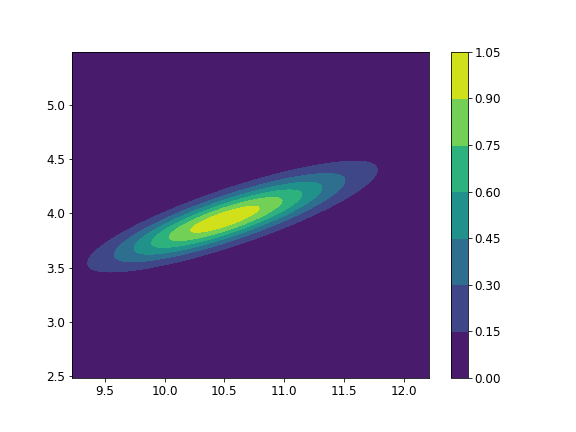
\includegraphics[width=70mm]{plots/logistic_regression_synthetic_true_posterior.png}
	& 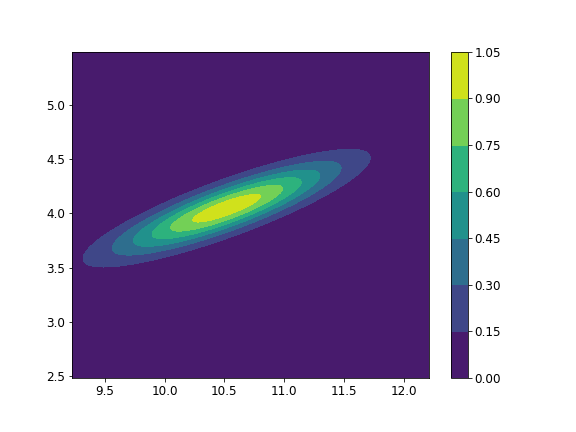
\includegraphics[width=70mm]{plots/logistic_regression_synthetic_vifa_posterior.png} \\
	(a) Ground truth
	& (b) VIFA \\[6pt]
\end{tabular}
\end{center}
\caption{The ground truth posterior pdf of a logistic regression model with two learnable parameters, plus the pdf of a FA model with a single latent dimension which was fit to the same data using VIFA. Both posteriors are scaled such that the maximum value is equal to $1$.}
\label{fig:logistic_regression_synthetic_data_posterior}
\end{figure}

\section{UCI Linear Regression Posterior Estimation}
\label{app:uci_posterior}
Table \ref{table:uci_datasets} shows the number of instances and input variables in each UCI regression dataset. Note that the original Energy Efficiency dataset has two target variables, heating load, and cooling load, but in these experiments, only the heating load was used.

\begin{table}[h!]
\caption{UCI regression datasets used in experiments.}
\begin{center}
\begin{tabular}{l|ll}
\label{table:uci_datasets}
\textbf{Dataset}              & \textbf{No. of Instances} & \textbf{No. of Input Variables} \\ \hline
Energy Efficiency             & 768                       & 8                               \\
Boston Housing                & 506                       & 13                              \\
Concrete Compressive Strength & 1030                      & 8                               \\
Yacht Hydrodynamics           & 308                       & 6                    
\end{tabular}
\end{center}
\end{table}

Table \ref{table:vifa_uci_hyperparameters} shows the hyperparameter values used in the experiments.
\begin{table}[h!]
\caption{VIFA hyperparameters for UCI linear regression experiments.}
\begin{center}
\label{table:vifa_uci_hyperparameters}
\begin{tabular}{l|lllllll}
\textbf{Dataset} & \textbf{$K$} & \textbf{Epochs} & \textbf{$M$} & \textbf{$L$} & \textbf{$\eta$} & \textbf{$\alpha$} & \textbf{$\beta$} \\ \hline
Energy Efficiency 				& 3 & 25,000 & 100 & 10 	& 0.01 	& 0.0608 & 0.1246 \\ 
Boston Housing 				& 3 & 25,000 & 100 & 10 	& 0.001 	& 0.2859 & 0.0429 \\
 Concrete Compressive Strength	& 3 & 20,000 & 100 & 10 	& 0.01 	& 0.0254 & 0.0101 \\
 Yacht Hydrodynamics 			& 3 & 45,000 & 100 & 10 	& 0.01 	& 0.0291 & 0.0114 \\
\end{tabular}
\end{center}
\end{table}

Recall that Section \ref{sec:experiments_on_UCI_datasets} presented qualitative comparisons of the true posterior of a linear regression model and the approximate posterior learned by VIFA for the Boston Housing and Yacht Hydrodynamics datasets. Figure \ref{fig:posterior_energy_efficiency} and Figure \ref{fig:posterior_concrete_strength} show the same comparisons for the Energy Efficiency and Concrete Compressive Strength datasets, respectively. Finally, Table \ref{table:linear_regression_vi_posterior_uci} contains quantitative measures of the difference between the true and estimate posteriors for all four UCI regression datasets. 

\begin{figure}[!htbp] 
	\begin{tabular}{c}
		\includegraphics[width=140mm]{plots/energy_efficiency_posterior_mean.png} \\
		(a) Comparison of true and estimated posterior means \\[6pt] 
		 \includegraphics[width=140mm]{plots/energy_efficiency_posterior_variance.png} \\
		(b) Comparison of true and estimated posterior variances \\[6pt] 
		\includegraphics[width=140mm]{plots/energy_efficiency_posterior_covariance.png} \\
		(c) Comparison of true and estimated posterior covariances \\[6pt] 
	\end{tabular}
	\caption{Comparison of the ground truth posterior of a linear regression model fit to the Energy Efficiency dataset, and the approximate posterior learned by VIFA. Variances and covariance are plotted separately due to the difference in their magnitude. In plot (c), the diagonal entries of the covariance matrices have been set to zero.}
	\label{fig:posterior_energy_efficiency}
\end{figure}

\begin{figure}[!htbp] 
	\begin{tabular}{c}
		\includegraphics[width=140mm]{plots/concrete_strength_posterior_mean.png} \\
		(a) Comparison of true and estimated posterior means \\[6pt] 
		 \includegraphics[width=140mm]{plots/concrete_strength_posterior_variance.png} \\
		(b) Comparison of true and estimated posterior variances \\[6pt] 
		\includegraphics[width=140mm]{plots/concrete_strength_posterior_covariance.png} \\
		(c) Comparison of true and estimated posterior covariances \\[6pt] 
	\end{tabular}
	\caption{Comparison of the ground truth posterior of a linear regression model fit to the Concrete Compressive Strength dataset, and the approximate posterior learned by VIFA. Variances and covariance are plotted separately due to the difference in their magnitude. In plot (c), the diagonal entries of the covariance matrices have been set to zero.}
	\label{fig:posterior_concrete_strength}
\end{figure} 

\begin{table}[!h]
\caption{For each UCI dataset, the distance between the true posterior distribution
of the parameter vector of a linear regression model and the approximate FA posterior
estimated by VIFA. Relative distances between the true and approximate means and
covariances are shown. Each relative distance is the Frobenius norm of the difference
between the true parameter and the approximate parameter divided by the Frobenius
norm of the true parameter. Also shown is the 2-Wasserstein distance between the true
posterior Gaussian distribution and the approximate Gaussian distribution, divided by
the number of dimensions in the dataset.}
\label{table:linear_regression_vi_posterior_uci}
\begin{center}
\begin{tabular}{l|lll}
\textbf{Dataset} & \textbf{Rel. Dist. from Mean} & \textbf{Rel. Dist. from Covar.} & \textbf{Scaled Wasserstein Dist.} \\ \hline
Energy           & 0.0051                        & 0.0421                          & 0.0564                            \\
Boston           & 0.0262                        & 0.3185                          & 0.0468                            \\
Concrete         & 0.0047                        & 0.0840                          & 0.0278                            \\
Yacht            & 0.0435                        & 0.0391                          & 0.1210                           
\end{tabular}
\end{center}
\end{table}

\section{UCI Logistic Regression Posterior Estimation}
\label{app:UCI_logistic_regression_posterior_estimation}

\subsection{Methodology and Discussion}

\textbf{Methodology} We picked the same four classification datasets as in SLANG \cite{mishkin2018}, that is Australian, Breast Cancer, a1a and USPS(3v5) \footnote{Downloaded from https://github.com/aaronpmishkin/SLANG/releases/download/v1.0.0/data.zip}. More details about these datasets are given in Appendix \ref{app:dataset_implementation_and_results_details}. The learning rate and number of epoches are tuned in the same way as in Section \ref{sec:experiments_on_UCI_datasets}. The latent dimension was set to $K = 5$ for all datasets. The mini-batch size and
Monte Carlo average size were set to M = 100 and L = 10, respectively, which are the same choices as in Section \ref{sec:experiments_on_UCI_datasets}. While training, gradient norms were clipped at a maximum value of 10. Bambi library \cite{Capretto2022} is in use for computing the ground truth posterior. 20,000 Markov Chain Monte Carlo (MCMC) iterations are adopted for Australian and Breast Cancer datasets, and 25,000 iterations are used for a1a and USPS(3v5) datasets.


\textbf{Results and Discussion}

Figures \ref{fig:posterior_Australian_and_a1a} show a qualitative comparison of the true posterior of a logistic regression model and the approximate posterior learned by VIFA, in the case of the Australian and the a1a datasets.  Qualitative comparisons for the other datasets can be found in Figures \ref{fig:posterior_Breast_Cancer} and \ref{fig:posterior_USPS} in Appendix \ref{app:dataset_implementation_and_results_details}, along with quantitative results for all four datasets in Table \ref{table:logistic_regression_vi_posterior_uci}. It is noticeable that the Australian and the a1a dataset have dimensions 14 and 123, but both approximated by VIFA has latent dimension equal to 5. In terms of the posterior mean, VIFA give good quality approximations for both datasets. The claim can be validated by examining Figure \ref{fig:posterior_Australian_and_a1a} (a) and (b), where the difference between the ground truth and the VIFA Approximation is not obvious. The relative distance of the approximate posterior mean from the ground truth for both the Australian dataset and the a1a dataset are small, which are 0.0215 and 0.0204 respectively. However, the approximation quality for variances and off-diagonal covariances are not as good as for the means. In terms of variances, one may notice clear difference between the ground truth and the VIFA Approximation in Figure \ref{fig:posterior_Australian_and_a1a} (c) and (d). The difference is more obvious for the comparison between covariances from VIFA approximation and ground truth covariances for the a1a dataset. This is understandable, since the a1a dataset is of high dimensional, a Factor analysis distribution with latent dimension being 5 might be not enough to capture its true posterior. In addition, the relative distance of the approximate posterior covariance from the ground truth is actually worse for the a1a: 0.3882 compared to 0.1018 for the Australian. 
This can be explained by a fact that the quality of the posterior covariance approximation is dependent on the data dimension relative to the latent dimension, which is already stated in Section \ref{sec:experiments_on_UCI_datasets}.

\begin{figure}[!htbp] 
\begin{center}
	\begin{tabular}{cc}
		\includegraphics[width=85mm]{plots/Australian_posterior_mean.png}
		& \includegraphics[width=85mm]{plots/a1a_posterior_mean.png} \\
        (a) Australian posterior mean
        & (b) a1a posterior mean \\
		\includegraphics[width=85mm]{plots/Australian_posterior_variance.png} 
        & \includegraphics[width=85mm]{plots/a1a_posterior_variance.png} \\
        (c) Australian posterior variance
        & (d) a1a posterior variance \\
        \includegraphics[width=85mm]
        {plots/Australian_posterior_covariance.png}
        & \includegraphics[width=85mm]
        {plots/a1a_posterior_covariance.png} \\
        (e) Australian posterior covariance
        & (f) a1a posterior covariance
        
	\end{tabular}
	\caption{Comparison of the ground truth posterior of logistic regression models fit the Australian and the a1a datasets, and the approximate posteriors learned by VIFA. Variances and covariance are plotted separately due to the difference in their magnitude. In plots (e) and (f), the diagonal entries of the covariance matrices have been set to zero. In each plot, the true covariance is placed on the left.}
	\label{fig:posterior_Australian_and_a1a}
\end{center}
\end{figure}

\subsection{Dataset, Implementation and More Results Details}
\label{app:dataset_implementation_and_results_details}
Table \ref{table:uci_classification_datasets} shows the number of instances and input variables in each UCI classification dataset. Note that we only use the training sets in original datasets in SLANG \cite{mishkin2018}.

\begin{table}[!h]
\caption{UCI classification datasets used in experiments.}
\label{table:uci_classification_datasets}
\begin{center}
\begin{tabular}{l|ll}
\textbf{Dataset}    & \textbf{No. of  Instances} & \textbf{No. of Input Variables}  \\ \hline
USPS3v5             & 767                        & 256                                                    \\
a1a                 & 1605                       & 123                                                \\
Australian-scale    & 345                        & 14                                                   \\
Breast-cancer-scale & 341                        & 10                                                  
\end{tabular}
\end{center}
\end{table}

Table \ref{table:vifa_uci_logistic_hyperparameters} shows the hyperparameter values used in the experiments. Note that the values of prior precision for the datasets are same SLANG \cite{mishkin2018}.

\begin{table}[!h]
\caption{VIFA hyperparameters for UCI logistic regression experiments.}
\label{table:vifa_uci_logistic_hyperparameters}
\begin{center}
\begin{tabular}{l|llllll}
\textbf{Dataset}    & \textit{K} & \textbf{Epochs} & M   & L  & $\eta$   & \textbf{Prior Precision} \\ \hline
USPS3v5             & 5          & 10,000          & 100 & 10 & 0.001 & 25                       \\
a1a                 & 5          & 30,000          & 100 & 10 & 0.001 & 2.8072                   \\
Australian-scale    & 5          & 30,000          & 100 & 10 & 0.001 & 1e-5                     \\
Breast-cancer-scale & 5          & 23,000          & 100 & 10 & 0.001 & 1.0                     
\end{tabular}
\end{center}
\end{table}

Figure \ref{fig:posterior_Breast_Cancer} and Figure \ref{fig:posterior_USPS} show the same comparisons for the Breast Cancer and USPS datasets, respectively. Finally, Table \ref{table:logistic_regression_vi_posterior_uci} contains quantitative measures of the difference between the true and estimate posteriors for all four classification datasets.

\begin{table}[!h]
\caption{For each UCI dataset, the distance between the true posterior distribution of the parameter vector of a logistic regression model and the approximate FA posterior estimated by VIFA. Relative distances between the true and approximate means and covariances are shown. Each relative distance is the Frobenius norm of the difference between the true parameter and the approximate parameter divided by the Frobenius norm of the true parameter. Also shown is the 2-Wasserstein distance between the true posterior Gaussian distribution and the approximate Gaussian distribution, divided by the number of dimensions in the dataset.}
\label{table:logistic_regression_vi_posterior_uci}
\begin{center}
\begin{tabular}{l|lll}
\textbf{Dataset}    & \textbf{Rel. Dist. from Mean} & \textbf{Rel. Dist. from Covar.} & \textbf{Scaled Wasserstein Dist.} \\ \hline
USPS3v5             & 0.4078                        & 0.5199                          & 0.0044                            \\
a1a                 & 0.0204                        & 0.3882                          & 0.0116                            \\
Australian-scale    & 0.0215                        & 0.1018                          & 0.0390                            \\
Breast-cancer-scale & 0.0205                        & 0.1729                          & 0.0297                           
\end{tabular}
\end{center}
\end{table}


\begin{figure}[!htbp] 
	\begin{tabular}{c}
		\includegraphics[width=140mm]{plots/Breast_Cancer_posterior_mean.png} \\
		(a) Comparison of true and estimated posterior means \\[6pt] 
		 \includegraphics[width=140mm]{plots/Breast_Cancer_posterior_variance.png} \\
		(b) Comparison of true and estimated posterior variances \\[6pt] 
		\includegraphics[width=140mm]{plots/Breast_Cancer_posterior_covariance.png} \\
		(c) Comparison of true and estimated posterior covariances \\[6pt] 
	\end{tabular}
	\caption{Comparison of the ground truth posterior of a logistic regression model fit to the Breast Cancer dataset, and the approximate posterior learned by VIFA. Variances and covariance are plotted separately due to the difference in their magnitude. In plot (c), the diagonal entries of the covariance matrices have been set to zero.}
	\label{fig:posterior_Breast_Cancer}
\end{figure}

\begin{figure}[!htbp] 
	\begin{tabular}{c}
		\includegraphics[width=140mm]{plots/USPS_posterior_mean.png} \\
		(a) Comparison of true and estimated posterior means \\[6pt] 
		 \includegraphics[width=140mm]{plots/USPS_posterior_variance.png} \\
		(b) Comparison of true and estimated posterior variances \\[6pt] 
		\includegraphics[width=140mm]{plots/USPS_posterior_covariance.png} \\
		(c) Comparison of true and estimated posterior covariances \\[6pt] 
	\end{tabular}
	\caption{Comparison of the ground truth posterior of a logistic regression model fit to the USPS dataset, and the approximate posterior learned by VIFA. Variances and covariance are plotted separately due to the difference in their magnitude. In plot (c), the diagonal entries of the covariance matrices have been set to zero.}
	\label{fig:posterior_USPS}
\end{figure}


\section{UCI Neural Network Regression Predictions}\label{app:uci_nn_predictions}

This section provides more details and results for the neural network prediction experiments in Section \ref{sec:uci_nn_predictions}. Firstly, important details which are worth making explicit are the loss functions used in the experiments. When training, the average negative log-likelihood term used on line 12 of Algorithm \ref{alg:vi_fa} was set to
\begin{equation}\label{eqn:train_nll}
	-\frac{1}{M} \sum_{(\vx, y) \in \mathcal{B}} \log \mathcal{N}\big(y; f(\vx; \vtheta), \beta^{-1}\big),
\end{equation}
where $\mathcal{B}$ is a mini-batch of $M$ training examples, $f(\vx; \vtheta)$ is the prediction of the neural network for input $\vx$ and parameters $\vtheta$ and $\beta$ is a hyperparameter. 

When testing, the marginal log-likelihood of a test example $(\vx, y)$ is
\begin{align}
\begin{split}
	\log p(y | \vx, \alpha, \beta, \mathcal{D}) 
	& = \log \int p(y | \vx, \vtheta, \beta) p(\vtheta | \alpha, \beta, \mathcal{D}) d\vtheta \\
	& = \log \int \mathcal{N}\big(y; f(\vx; \vtheta), \beta^{-1}\big) p(\vtheta | \alpha, \beta, \mathcal{D}) d\vtheta,
\end{split}
\end{align}
where $\mathcal{D}$ is the training data and $p(\vtheta | \alpha, \beta, \mathcal{D})$ is the approximate posterior learned by VIFA or SLANG for hyperparameters $\alpha$ and $\beta$. This integral cannot be computed exactly. Instead, it was approximated by a sample average. Formally, 
\begin{align}
\begin{split}
	\log p(y | \vx, \alpha, \beta, \mathcal{D}) 
	& \approx \log \Bigg( \frac{1}{L} \sum_{l=1}^L \mathcal{N}\big(y; f(\vx; \vtheta_l), \beta^{-1}\big) \Bigg) \\
	& = \log \Bigg( \sum_{l=1}^L \mathcal{N}\big(y; f(\vx; \vtheta_l), \beta^{-1}\big) \Bigg) - \log L,
\end{split}
\end{align}
where each $\vtheta_l \sim p(\vtheta | \alpha, \beta, \mathcal{D})$. This quantity was averaged over the full test set to approximate the average marginal log-likelihood. In addition, the test root mean squared error (RMSE) was also computed, where the squared error of a single test example is
\begin{equation}
	\Bigg(y - \frac{1}{L} \sum_{l=1}^L f(\vx; \vtheta_l)\Bigg)^2.
\end{equation}
When computing these metrics, the Monte Carlo average size was set to $L=100$.

Recall that Table \ref{table:neural_nets_uci_mean} provides the test metrics for the experiments averaged over 20 different train-test splits. The corresponding median results are given in Table \ref{table:neural_nets_uci_median}.

\begin{table}[!h]
\caption{Median test results for prediction experiments with UCI regression datasets. Metrics are the average negative marginal log-likelihood (NMLL) and root mean squared error (RMSE). LR and NN refer to linear regression and neural networks, respectively. The median results over 20 different train-test splits are shown. The best results on each row are highlighted in bold.}
\label{table:neural_nets_uci_median}
\begin{center}
\begin{tabular}{l|llll}
\textbf{Metric} & \textbf{Dataset} & \textbf{VIFA-LR} & \textbf{VIFA-NN} & \textbf{SLANG-NN} \\ \hline
NMLL 	& Energy 		& $2.57$ 					& $2.54$ 					& $\mathbf{1.19}$ \\ 	
		& Boston   	& $2.88$	 				& $\mathbf{2.65}$ 			& $2.68$ \\ 			
		& Concrete	& $3.76$ 					& $3.33$ 					& $\mathbf{3.32}$ \\ 			
 	& Yacht    		& $3.62$ 					& $2.38$ 					& $\mathbf{1.59}$ \\ \hline
RMSE 	& Energy 	 	& $3.04$ 					& $2.93$ 					& $\mathbf{1.19}$ \\ 
		& Boston 	 	& $4.31$ 					& $\mathbf{3.51}$ 			& $6.47$ \\ 
		& Concrete  	& $10.27$ 				& $\mathbf{6.77}$ 			& $9.03$ \\ 
 	& Yacht 		& $9.07$ 					& $2.59$ 					& $\mathbf{1.21}$ \\ 
\end{tabular}
\end{center}
\end{table}

\section{Experiments on Medical Imaging Dataset}
\subsection{Definitions of Uncertainty Scores}\label{app:uncertainty_scores_defs}
Recall these are different ways to reflect predictive uncertainty. One definition adopted in \citet{band2022benchmarking} is that for any given test sample $\vx_*$ the predictive uncertainty is equal to the entropy of the predictive distribution: 
\begin{equation}
H(\E_{\vtheta \sim Q(\vtheta)}[p(\ry_* \mid f(\vx_* ; \vtheta))])=-\sum_{c \in\{0,1\}} \E_{\vtheta \sim Q(\vtheta)}[p(\ry_*=c \mid f(\vx_* ; \vtheta))] \log \E_{\vtheta \sim Q(\vtheta)} [p(\ry_*=c \mid f(\vx_* ; \vtheta))]
\end{equation}

where $H$ represents the Shannon entropy, $f(\vx_*;\vtheta)$ is logit value, $p(\ry_*=c \mid f(\vx_* ; \vtheta))$ is a binary cross-entropy likelihood function and $Q(\vtheta)$ is the variational distribution. In practice, the expectation $\E_{\vtheta \sim Q(\vtheta)}[p(\ry_* \mid f(\vx_* ; \vtheta))]$ is approximated by $S$ Monte Carlo samples,
$\E_{\vtheta \sim Q(\vtheta)}[p(\ry_* \mid f(\vx_* ; \vtheta))] \approx \frac{1}{S} \sum_i^S p(\ry_* \mid f(\vx_* ; \vtheta^{(i)}))$ , here $\{\vtheta^{(i)}\}_{i=1}^S$ are sampled from (trained) variational distribution $Q(\vtheta)$, and $p(\ry_* \mid f(\vx_* ; \vtheta^{(i)}))$ denotes the predictive distribution given parameter realization $\vtheta^{\left(i\right)}$.

Another way to define predictive uncertainty is by measuring the model disagreement \citep{d2021repulsive}, which is computed as:
\begin{equation}
    \mathcal{MD}^2 (\vx_*) = \sum_{c \in\{0,1\}} \E_{\vtheta \sim Q(\vtheta)}[(p(\ry_*=c \mid f(\vx_*; \vtheta)) - \E_{\vtheta \sim Q(\vtheta)}[p(\ry_* = c\mid f(\vx_* ; \vtheta))])^2]
\end{equation}
This quality represents how much 'disagreement' exist among the distribution of models. In practice, this quantity is approximated by $\mathcal{MD}^2(\vx_*) \approx \sum_{c \in\{0,1\}} \frac{1}{S}\sum_{\vtheta^{(i)} \in\{\vtheta^{(1)},...,\vtheta^{(S)}\}} (p(\ry_*=c \mid f(\vx_*; \vtheta^{(i)})) - \frac{1}{S}\sum_{\vtheta^{(i)} \in\{\vtheta^{(1)},...,\vtheta^{(S)}\}}[p(\ry_* = c\mid f(\vx_* ; \vtheta^{(i)}))])^2$, where $\{\vtheta^{(1)},...,\vtheta^{(S)}\}$ are Monte Carlo samples from the variational distribution $Q(\vtheta)$. It is easy to see if all models agree on the prediction $\vx_*$, the disagreement measures $\mathcal{MD}^2 (\vx_*)$ becomes zero. On the other hand, the larger the score $\mathcal{MD}^2 (\vx_*)$, the server disagreement exists between predictive distributions.


\subsection{Uncertainty on Medical Imaging}
\label{app:uncertainty_on_medical_imaging}
\begin{table}[!htp]
\caption{Mean F1-scores of selective prediction under different uncertainty levels. Uncertainty scores calculated from two distinct approaches are employed, which are predictive entropy and model disagreement. Test samples are arranged in ascending order based on their uncertainty scores. 'Proportion of Samples' indicates the percentage of ordered samples used for testing. Subset with smaller proportion indicates
its samplers have lower uncertainty scores. The results for F1 scores include standard errors. The best results in each column are highlighted in bold.}
\label{table: VIFA_uncertainty_f1_score}
\begin{center}
\begin{tabular}{c|cc}
\textbf{Proportion of Samples} & \textbf{Predictive Entropy} & \textbf{Model Disagreement} \\ \hline
\textbf{90\%}                               & 0.946$\pm$0.007                 & 0.945$\pm$0.007                 \\
\textbf{80\%}                               & 0.965$\pm$0.005                 & 0.966$\pm$0.004                 \\
\textbf{70\%}                               & 0.975$\pm$0.004                 & 0.976$\pm$0.004                 \\
\textbf{60\%}                               & 0.986$\pm$0.003                 & 0.985$\pm$0.003                 \\
\textbf{50\%}                               & \textbf{0.989$\pm$0.002}                 & \textbf{0.989$\pm$0.002}                
\end{tabular}
\end{center}
\end{table}


\begin{table}[!htp]
\caption{Mean AU-ROC scores of selective prediction under different uncertainty levels. Uncertainty scores calculated from two distinct approaches are employed, which are predictive entropy and model disagreement. Test samples are arranged in ascending order based on their uncertainty scores. 'Proportion of Samples' indicates the percentage of ordered samples used for testing. Subset with smaller proportion indicates
its samplers have lower uncertainty scores. The results for AU-ROC include standard errors. The best results in each column are highlighted in bold.}
\label{table: VIFA_uncertainty_auroc}
\begin{center}
\begin{tabular}{c|cc}
\textbf{Proportion of Samples} & \textbf{Predictive Entropy} & \textbf{Model Disagreement} \\ \hline
\textbf{90\%}                               & 0.984$\pm$0.002                 & 0.984$\pm$0.003                 \\
\textbf{80\%}                               & 0.989$\pm$0.002                 & 0.989$\pm$0.002                 \\
\textbf{70\%}                               & 0.992$\pm$0.002                 & 0.992$\pm$0.002                 \\
\textbf{60\%}                               & 0.994$\pm$0.002                 & 0.994$\pm$0.002                 \\
\textbf{50\%}                               & \textbf{0.995$\pm$0.001}                 & \textbf{0.995$\pm$0.002}                
\end{tabular}
\end{center}
\end{table}


\end{document}
